\documentclass[12pt,twoside]{report}

%%%%%%%%%%%%%%%%%%%%%%%%%%%%%%%%%%%%%%%%%%%%%%%%%%%%%%%%%%%%%%%%%%%%%%%%%%%%%

% Definitions for the title page
% Edit these to provide the correct information

\newcommand{\reporttitle}{Competición en Kaggle}
\newcommand{\reportauthor}{David}
\newcommand{\degreetype}{Doble Grado Ingeniería Informática y Matemáticas}
\newcommand{\labgroup}{Grupo 2 de prácticas}
\newcommand{\email}{}

%%%%%%%%%%%%%%%%%%%%%%%%%%%%%%%%%%%%%%%%%%%%%%%%%%%%%%%%%%%%%%%%%%%%%%%%%%%%%

% load some definitions and default packages
%%%%%%%%%%%%%%%%%%%%%%%%%%%%%%%%%%%%%%%%%
% University Assignment Title Page 
% LaTeX Template
% Version 1.0 (27/12/12)
%
% This template has been downloaded from:
% http://www.LaTeXTemplates.com
%
% Original author:
% WikiBooks (http://en.wikibooks.org/wiki/LaTeX/Title_Creation)
%
% License:
% CC BY-NC-SA 3.0 (http://creativecommons.org/licenses/by-nc-sa/3.0/)
% 
%
%%%%%%%%%%%%%%%%%%%%%%%%%%%%%%%%%%%%%%%%%
%----------------------------------------------------------------------------------------
%	PACKAGES AND OTHER DOCUMENT CONFIGURATIONS
%----------------------------------------------------------------------------------------
\usepackage[a4paper,hmargin=2.8cm,vmargin=2.0cm,includeheadfoot]{geometry}
\usepackage{textpos}
\usepackage{tabularx,longtable,multirow,subfigure,caption}%hangcaption
\usepackage{fncylab} %formatting of labels
\usepackage{fancyhdr} % page layout
\usepackage{url} % URLs
\usepackage[english]{babel}
\usepackage{amsmath}
\usepackage{graphicx}
\usepackage{dsfont}
\usepackage{epstopdf} % automatically replace .eps with .pdf in graphics
\usepackage{array}
\usepackage{latexsym}
\usepackage{booktabs}
\usepackage[pdftex,hypertexnames=false,colorlinks]{hyperref} % provide links in pdf
\usepackage[
    type={CC},
    modifier={by-nc-sa},
    version={3.0},
]{doclicense}
\usepackage[
backend=bibtex,
style=alphabetic,
sorting=ynt
]{biblatex}
\addbibresource{refs.bib}

\usepackage{listings}
\usepackage{color}
\usepackage{multicol}
\definecolor{dkgreen}{rgb}{0,0.6,0}
\definecolor{gray}{rgb}{0.5,0.5,0.5}
\definecolor{mauve}{rgb}{0.58,0,0.82}

\lstset{frame=tb,
  language=Python,
  aboveskip=0.5mm,
  belowskip=0.5mm,
  showstringspaces=false,
  columns=flexible,
  basicstyle={\small\ttfamily},
  numbers=none,
  numberstyle=\tiny\color{gray},
  keywordstyle=\color{blue},
  commentstyle=\color{dkgreen},
  stringstyle=\color{mauve},
  breaklines=true,
  breakatwhitespace=true,
  tabsize=1
}

\hypersetup{pdftitle={},
  pdfsubject={}, 
  pdfauthor={},
  pdfkeywords={}, 
  pdfstartview=FitH,
  pdfpagemode={UseOutlines},% None, FullScreen, UseOutlines
  bookmarksnumbered=true, bookmarksopen=true, colorlinks,
    citecolor=black,%
    filecolor=black,%
    linkcolor=black,%
    urlcolor=black}

\usepackage[all]{hypcap}


%\usepackage{color}
%\usepackage[tight,ugly]{units}
\usepackage{float}
%\usepackage{tcolorbox}
%\usepackage[colorinlistoftodos]{todonotes}
% \usepackage{ntheorem}
% \theoremstyle{break}
% \newtheorem{lemma}{Lemma}
% \newtheorem{theorem}{Theorem}
% \newtheorem{remark}{Remark}
% \newtheorem{definition}{Definition}
% \newtheorem{proof}{Proof}


%%% Default fonts
\renewcommand*{\rmdefault}{bch}
\renewcommand*{\ttdefault}{cmtt}
\renewcommand{\contentsname}{Índice}

%%% Default settings (page layout)
\setlength{\parindent}{0em}  % indentation of paragraph

\setlength{\headheight}{14.5pt}
\pagestyle{fancy}
\renewcommand{\chaptermark}[1]{\markboth{\chaptername\ \thechapter.\ #1}{}} 

\fancyfoot[ER,OL]{\sffamily\textbf{\thepage}}%Page no. in the left on odd pages and on right on even pages
\fancyfoot[OC,EC]{\sffamily }
\renewcommand{\headrulewidth}{0.1pt}
\renewcommand{\footrulewidth}{0.1pt}
\captionsetup{margin=10pt,font=small,labelfont=bf}


%--- chapter heading

\def\@makechapterhead#1{%
  \vspace*{10\p@}%
  {\parindent \z@ \raggedright \sffamily
    \interlinepenalty\@M
    \Huge\bfseries \thechapter \space\space #1\par\nobreak
    \vskip 30\p@
  }}

%---chapter heading for \chapter*  
\def\@makeschapterhead#1{%
  \vspace*{10\p@}%
  {\parindent \z@ \raggedright
    \sffamily
    \interlinepenalty\@M
    \Huge \bfseries  #1\par\nobreak
    \vskip 30\p@
  }}

\allowdisplaybreaks

% load some macros
% Here, you can define your own macros. Some examples are given below.

\newcommand{\R}[0]{\mathds{R}} % real numbers
\newcommand{\Z}[0]{\mathds{Z}} % integers
\newcommand{\N}[0]{\mathds{N}} % natural numbers
\newcommand{\C}[0]{\mathds{C}} % complex numbers
\renewcommand{\vec}[1]{{\boldsymbol{{#1}}}} % vector
\newcommand{\mat}[1]{{\boldsymbol{{#1}}}} % matrix


\date{Curso 2020-2021}

\begin{document}

% load title page
% Last modification: 2015-08-17 (Marc Deisenroth)
\begin{titlepage}

\newcommand{\HRule}{\rule{\linewidth}{0.5mm}} % Defines a new command for the horizontal lines, change thickness here


%----------------------------------------------------------------------------------------
%	LOGO SECTION
%----------------------------------------------------------------------------------------


\includegraphics[width = 4cm]{../notebooks/figures/ugr}\\[0.5cm] 

\center % Center remainder of the page

%----------------------------------------------------------------------------------------
%	HEADING SECTIONS
%----------------------------------------------------------------------------------------

\textsc{\Large Universidad de Granada}\\[0.5cm] 
\textsc{\large Práctica 3 Inteligencia de Negocio}\\[0.5cm] 

%----------------------------------------------------------------------------------------
%	TITLE SECTION
%----------------------------------------------------------------------------------------

\HRule \\[0.4cm]
{ \huge \bfseries \reporttitle}\\ % Title of your document
\HRule \\[1.5cm]
 
%----------------------------------------------------------------------------------------
%	AUTHOR SECTION
%----------------------------------------------------------------------------------------

\begin{minipage}{0.4\textwidth}
\begin{flushleft} \large
\reportauthor % Your name
\end{flushleft}
\end{minipage}
~


%----------------------------------------------------------------------------------------
%	FOOTER & DATE SECTION
%----------------------------------------------------------------------------------------
\vfill % Fill the rest of the page with whitespace
\labgroup\\
\email\\
\degreetype\\[0.5cm]

\makeatletter
\@date 
\makeatother


\end{titlepage}



% page numbering etc.
\pagenumbering{roman}
\clearpage{\pagestyle{empty}\cleardoublepage}
\setcounter{page}{1}
\pagestyle{fancy}


\clearpage{\pagestyle{empty}\cleardoublepage}

%%%%%%%%%%%%%%%%%%%%%%%%%%%%%%%%%%%%
%--- table of contents

Leaderboard final de la competición, \textbf{posición 10} con una score de \textbf{0.80586}.
\\
\\
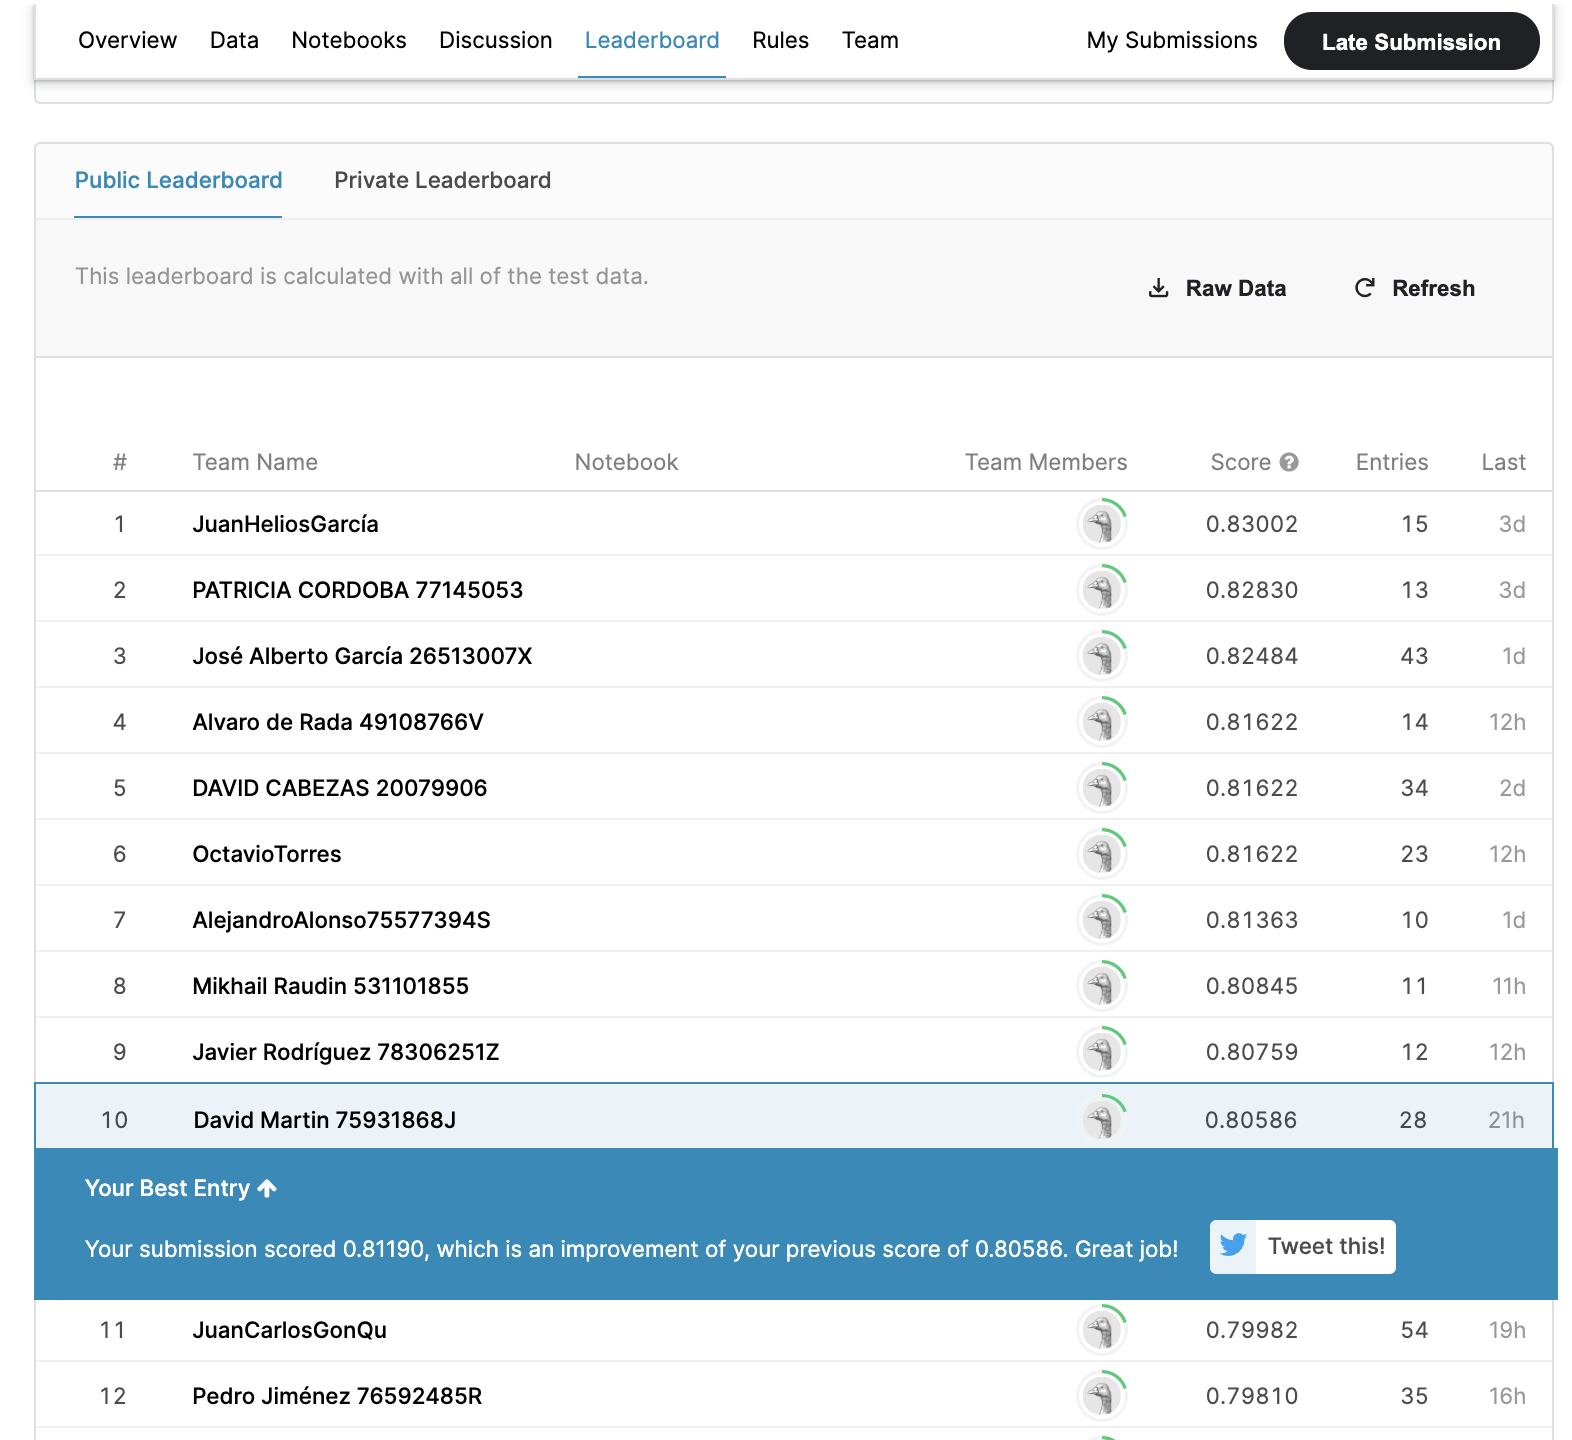
\includegraphics[width = \textwidth]{../notebooks/figures/leaderboard}\\

Podríamos haber conseguido más si hubieramos hecho subidas de ficheros con más cabeza ya que después redactar las documentación probando alguna cosa más (late submissions) conseguimos scores de hasta \textbf{0.81190}.
\\
\\
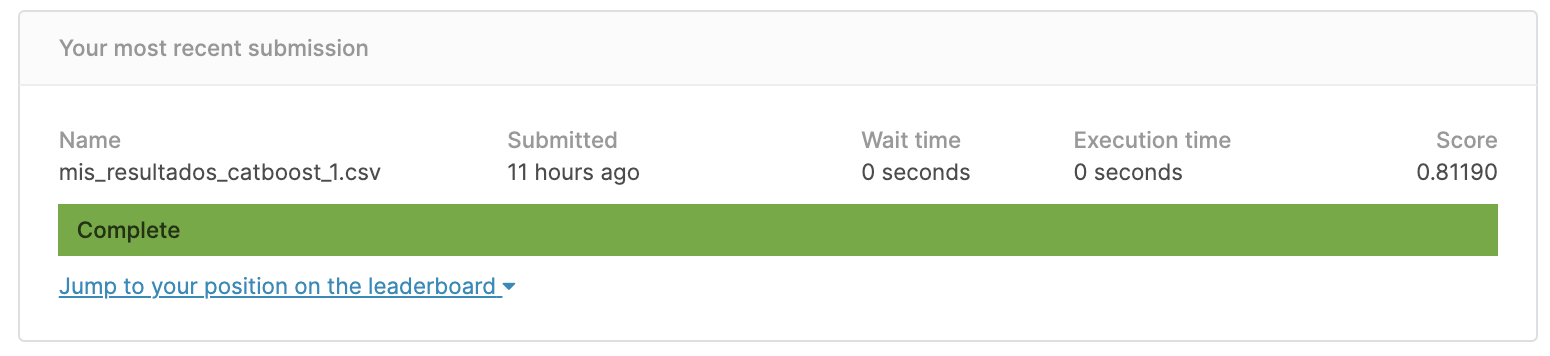
\includegraphics[width = \textwidth]{../notebooks/figures/late}\\

\fancyhead[RE,LO]{\sffamily {Table of Contents}}
\begingroup
\pagestyle{plain}
\tableofcontents 
\listoffigures
\listoftables
\endgroup

%\listoftables
\clearpage{\pagestyle{empty}\cleardoublepage}
\pagenumbering{arabic}
\setcounter{page}{1}
\fancyhead[LE,RO]{\slshape \rightmark}
\fancyhead[LO,RE]{\slshape \leftmark}


\chapter*{Introducción}
\addcontentsline{toc}{chapter}{Introducción}  

En esta tercera y última práctica de la asignatura Inteligencia de Negocio veremos el uso de métodos avanzados para aprendizaje supervisado en clasificación sobre una competición disponible en \textit{Kaggle}, creada ex-proceso para esta práctica. Se buscará adquirir destrezas para mejorar la capacidad predictiva del modelo mientras nos familiarizamos con una de las plataformas más  populares de competición en ciencias de datos.

\section*{Descripción del problema}
\addcontentsline{toc}{section}{Descripción del problema}  

En este problema existen datos de una serie de coches vendidos, y se han clasificado los coches en 5 categorías de precio. Se desea predecir la categoría del precio del coche, por lo que es un problema de clasificación multiclase.

El conjunto de entrenamiento consta de alrededor de 6000 instancias, y 14 atributos (de los cuales, id toma valores únicos y solo sirve para identificar cada ejemplo) con datos categóricos y enteros. Se trata de predecir la variable ordinal \textbf{Precio\_cat}, que representa el grado de coste que supone. Hay cinco valores: \textbf{1}, representa a los más baratos; \textbf{2}, representa aquellos baratos pero menos; \textbf{3}, representa a los que están en precio promedio; \textbf{4}, representa a los que son más caros que el promedio, y \textbf{5}, que representa a los coches más caros. Para medir el rendimiento de nuestros algoritmos, la competición usará la medida de precisión (accuracy), aunque se podrá utilizar otras medidas o criterios para identificar los algoritmos más promedores en la memoria.

\section*{Descripción de los atributos}
\addcontentsline{toc}{section}{Descripción de los atributos}  

A continuación se detalla el significado de los distintos atributos:
\begin{itemize}
	\item Nombre del tipo de coche
	\item Año del coche
	\item Kilómetros recorridos
	\item Combustible del coche (Petrol, Diesel, Electric, LPG y CNG)
	\item Tipo de marcha del coche (Manual y Automatic).
	\item Mano si es primera mano (First), Segunda (Second), Tercera (Third) y cuarta o más (Fourth \& Above).
 	\item Consumo en kilómetros por litro (kmpl).
 	\item MotorCC medido en centrómetros cúbicos (CC).
 	\item Potencia del motor medido (bhc).
 	\item Asientos
 	\item Descuento realizado por oferta especial (en porcentaje).
\end{itemize} 

\section*{Ficheros}
\addcontentsline{toc}{section}{Ficheros}  

Para trabajar se dispone de varios ficheros descargables en la página web de la competición:
\begin{itemize}
	\item train.csv: Fichero con todos los atributos, incluyendo el objetivo a predecir. Es el conjunto de datos que se puede usar para realizar el aprendizaje automático. Además, se deberá de evaluar usando validación cruzada para identificar los algoritmos más prometedores, y realizar el proceso de tuning que se considere. Se deberá de aplicar las técnicas de pre-procesamiento que se consideren interesantes.
	\item test.csv: Fichero con las instancias a predecir. Posee el mismo formato que train.csv, a excepción del atributo Precio cat, que evidentemente no aparece.
	\item sample.csv: Fichero con el formato del fichero a someter, que contiene únicamente el id y los valores de Precio cat.
\end{itemize}

También se ofrece un fichero para cada atributo de cara a facilitar una correcta etiquetación y normalización (que debería de aplicarse por igual a los datos de ambos ficheros) 

\chapter*{Competición}
\addcontentsline{toc}{chapter}{Competición}  

En esta parte de la documentación se explicarán las estrategias seguidas y el progreso que se ha ido desarrollando durante la competición. Para comenzar, haremos un poco de \textbf{EDA} para ver nuestros atributos (\textit{Exploratory data analysis}),  veremos distintos tipos de \textbf{preprocesamiento} que se plantean y describiremos los principales \textbf{algoritmos} para la predicción multiclase utilizados, haciendo mención especial en un apartado a una \textbf{red neuronal} creada para este problema.

Finalmente mostraremos una \textbf{tabla} [\ref{tab:tabla-scores}] con el conjunto de planteamientos que han sido más existosos (ya que la mayoría de subidas de ficheros han sido probando el mismo preprocesamiento pero usando distintos algoritmos), incluyendo la fecha de subida de Kaggle, la posición en el leader en ese momento, el preprocesamiento utilizando,  la puntuación de validación cruzada de 5 particiones respecto al conjunto de train.csv \footnote{el fichero \textbf{train.csv}, a su vez dividido en conjuntos de train y test y realizando validación cruzada de 5 particiones \textbf{únicamente} sobre el conjunto de train resultante de dividir el conjunto de train, puede ser un poco confuso, básicamente es que no combinamos train\_test} y la puntuación obtenida en Kaggle resultante al subir el fichero con la predicción realizada sobre el conjunto test.csv.

Por simplicidad y para hacer la tabla más cómoda visualmente, mostraremos únicamente los planteamientos más interesantes, ya que personalmente opino que no tiene mucho sentido añadir todas las subidas donde algunas son distintas combinaciones para distintos preprocesamientos, si tenemos una subida que considera un conjunto de  preprocesamientos y consigue una puntuación mejor que otros aplicados individualmente (por ejemplo, si en un intento hemos tratado con valores perdidos, y en otro intento hemos tratado de la misma manera valores perdidos y además hemos utilizado técnicas para el balanceo, únicamente pondremos el segundo intento ya que el primero es redundante).

\section*{Exploratory data analysis}
\addcontentsline{toc}{section}{Exploratory data analysis}

Todo lo relevante para recrear esta parte visual se encuentra al inicio del notebook \textbf{vanilla.ipynb}. Obteniendo información sobre nuestras variables

\begin{multicols}{2}
train.csv
\begin{lstlisting}
RangeIndex: 4819 entries, 0 to 4818
Data columns (total 14 columns):
 #   Column        Non-Null Count  Dtype  
---  ------        --------------  -----  
 0   id            4747 non-null   float64
 1   Nombre        4747 non-null   object 
 2   Ciudad        4747 non-null   object 
 3   Anio           4747 non-null   float64
 4   Kilometros    4747 non-null   float64
 5   Combustible   4747 non-null   object 
 6   Tipo_marchas  4747 non-null   object 
 7   Mano          4747 non-null   object 
 8   Consumo       4746 non-null   object 
 9   Motor_CC      4718 non-null   object 
 10  Potencia      4644 non-null   object 
 11  Asientos      4713 non-null   float64
 12  Descuento     659 non-null    float64
 13  Precio_cat    4819 non-null   int64  
dtypes: float64(5), int64(1), object(8)
\end{lstlisting}
\columnbreak
test.csv
\begin{lstlisting}
RangeIndex: 1159 entries, 0 to 1158
Data columns (total 13 columns):
 #   Column        Non-Null Count  Dtype  
---  ------        --------------  -----  
 0   id            1159 non-null   int64  
 1   Nombre        1159 non-null   object 
 2   Ciudad        1159 non-null   object 
 3   Anio           1159 non-null   int64  
 4   Kilometros    1159 non-null   int64  
 5   Combustible   1159 non-null   object 
 6   Tipo_marchas  1159 non-null   object 
 7   Mano          1159 non-null   object 
 8   Consumo       1159 non-null   object 
 9   Motor_CC      1159 non-null   object 
 10  Potencia      1159 non-null   object 
 11  Asientos      1159 non-null   float64
 12  Descuento     155 non-null    float64
dtypes: float64(2), int64(3), object(8)
\end{lstlisting}
\end{multicols}

Hacemos una primera vista a las variables numéricas de nuestro dataset en modo de histograma [\ref{fig:features-distribucions}], donde se aprecia la presencia de outliers, por ejemplo en el caso de nuestro atributo \textbf{kilómetros} y asimetría en las distribuciones (\textit{skewed data}).

\begin{figure}[H]
\caption{Histograma general}
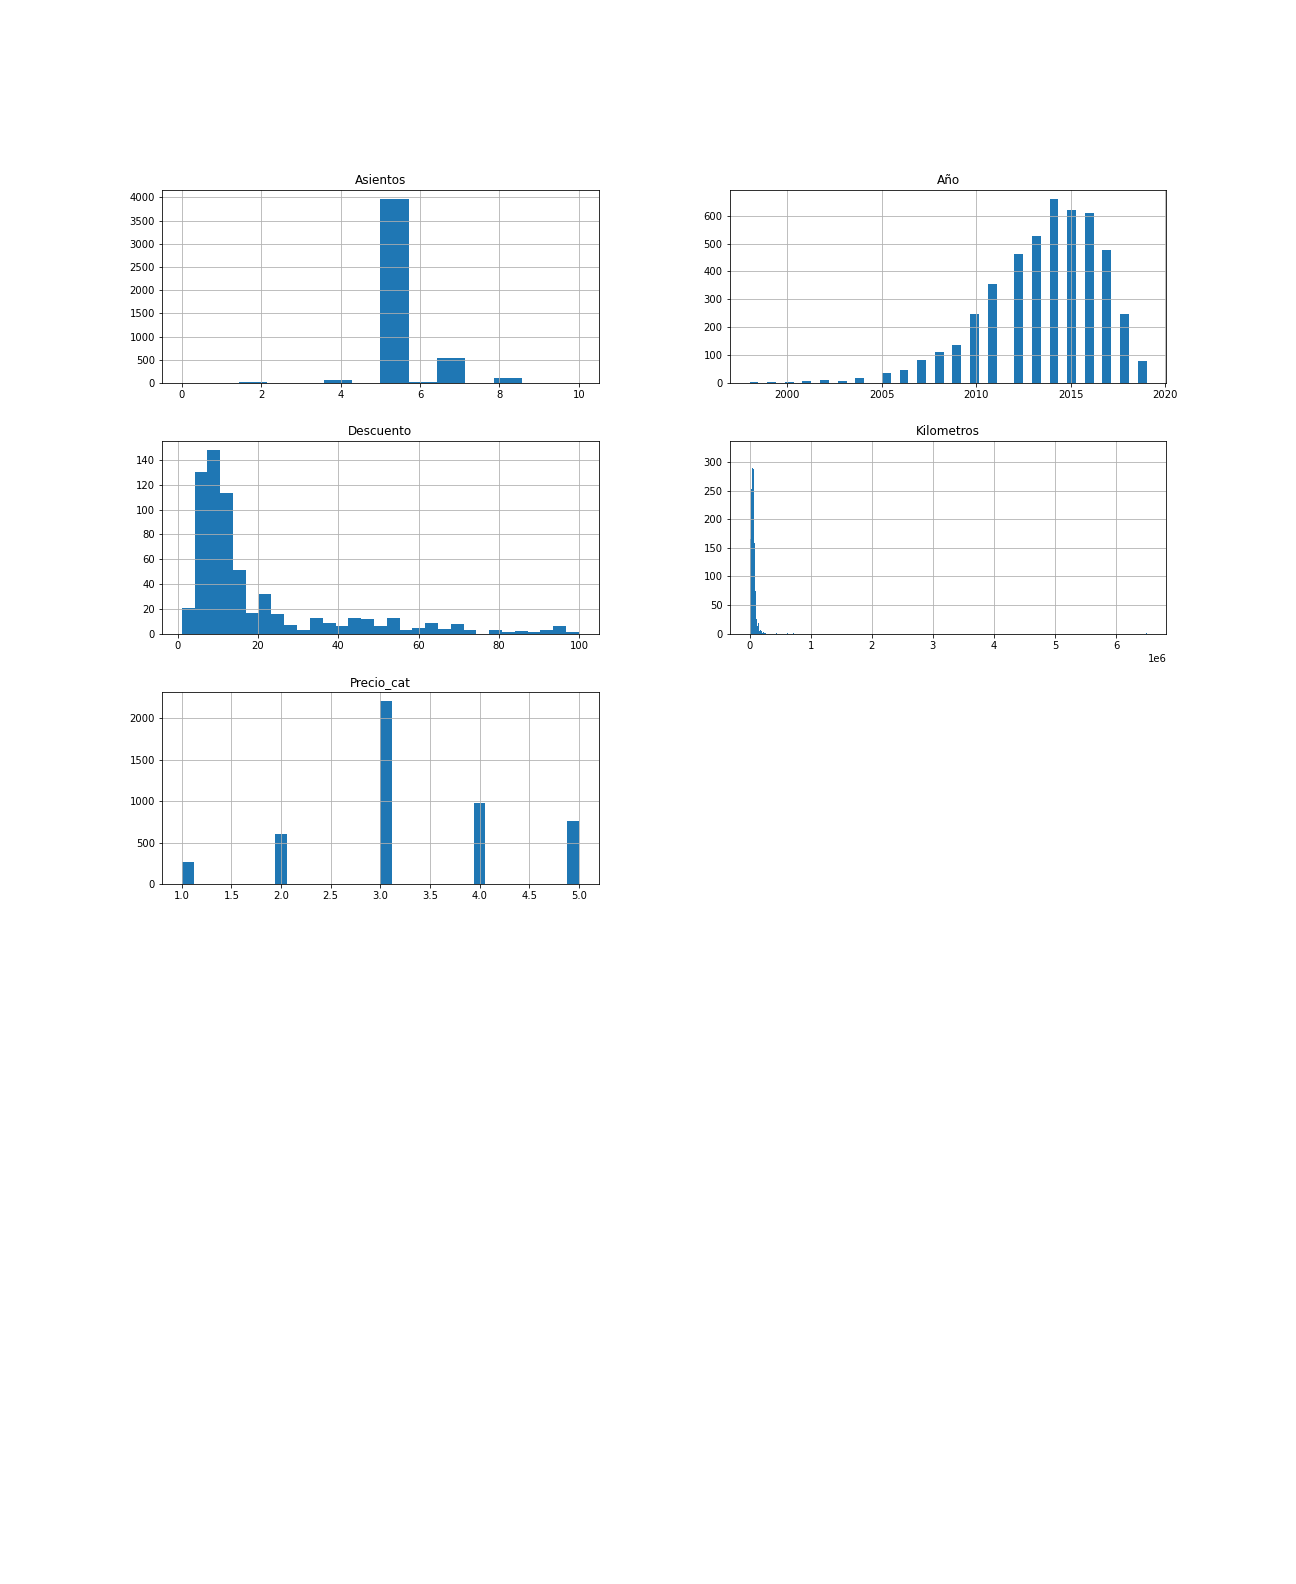
\includegraphics[width=\textwidth]{../notebooks/figures/hist.png}
\label{fig:features-distribucions}
\end{figure}

Vamos a mostrar visualizaciones de algunas variables discretas individualmente y respecto a nuestra variable a predecir \textbf{Precio\_cat} en la figura [\ref{fig:eda_discretes}], también en la figura [\ref{fig:eda_anio_precio}] vemos algo esperado y es la influencia del atributo Año en la variable a predecir, ya que con el tiempo los coches valen menos.


\begin{figure}[H]
\begin{multicols}{2}
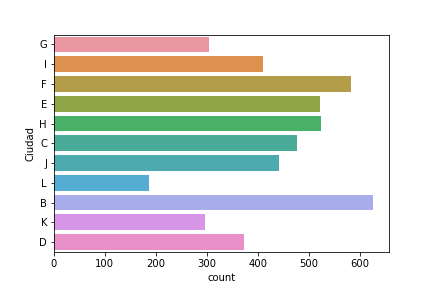
\includegraphics[width=8cm]{../notebooks/figures/ciudad.png}
\columnbreak
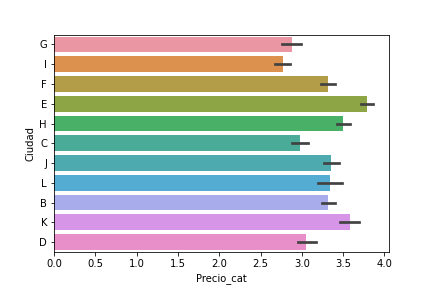
\includegraphics[width=8cm]{../notebooks/figures/ciudad_precio_cat.png}
\end{multicols}
\caption{Ciudad vs Precio\_cat}

\begin{multicols}{2}
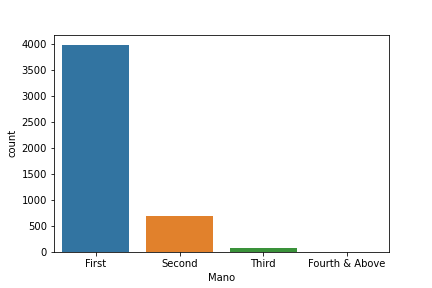
\includegraphics[width=8cm]{../notebooks/figures/mano.png}
\columnbreak
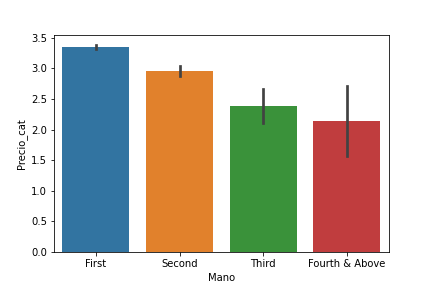
\includegraphics[width=8cm]{../notebooks/figures/mano_precio_cat.png}
\end{multicols}
\caption{Mano vs Precio\_cat}

\begin{multicols}{2}
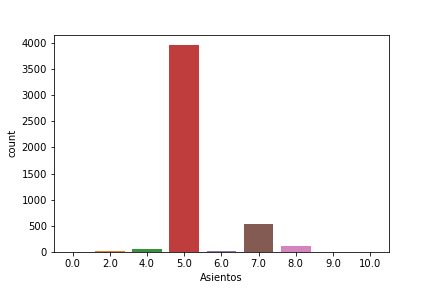
\includegraphics[width=8cm]{../notebooks/figures/asientos.png}
\columnbreak
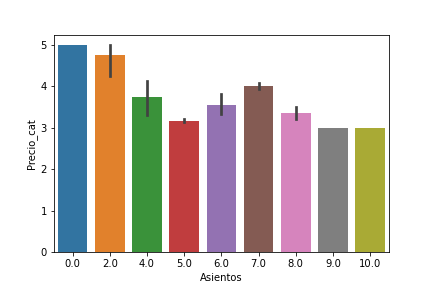
\includegraphics[width=8cm]{../notebooks/figures/asientos_precio_cat.png}
\end{multicols}
\caption{Asientos vs Precio\_cat}
\label{fig:eda_discretes}
\end{figure}


\begin{figure}[H]
\begin{multicols}{2}
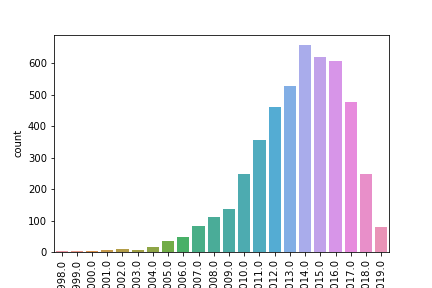
\includegraphics[width=8cm]{../notebooks/figures/anio.png}
\columnbreak
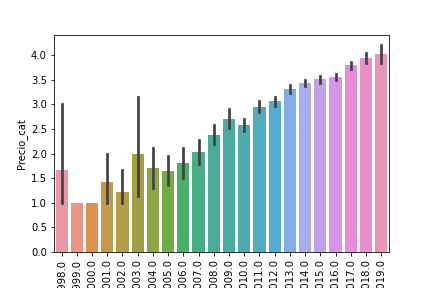
\includegraphics[width=8cm]{../notebooks/figures/anio_precio_cat.png}
\end{multicols}
\caption{Año vs Precio\_cat}
\label{fig:eda_anio_precio}
\end{figure}


Destacamos el caso de Asientos, donde hay una gran cantidad de coches con 5 asientos pero a su vez son de los que menos precio valen, esto puede deberse debido a la oferta y demanda.

A su vez, para visualizar también las variables de objetos como Combustible, Consumo etc que tienen un parámetro numérico junto a la medida, preprocesamos estos atributos dejandolo solo el valor numérico para poder visualizarlo, vemos en la figura [\ref{fig:dis_atributos}] visualizaciones de estas variables preprocesadas de la manera comentada junto a un boxplot.

\begin{figure}[H]
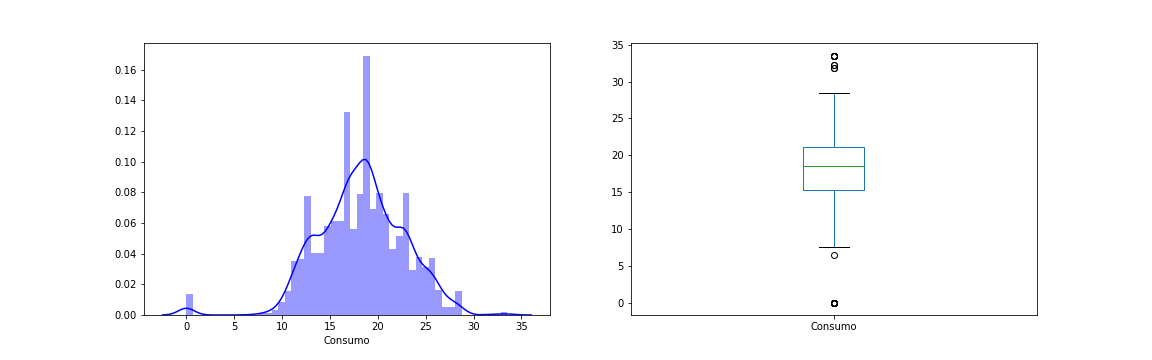
\includegraphics[width=\textwidth]{../notebooks/figures/consumo_dis.png}
\caption{Distribución Consumo}
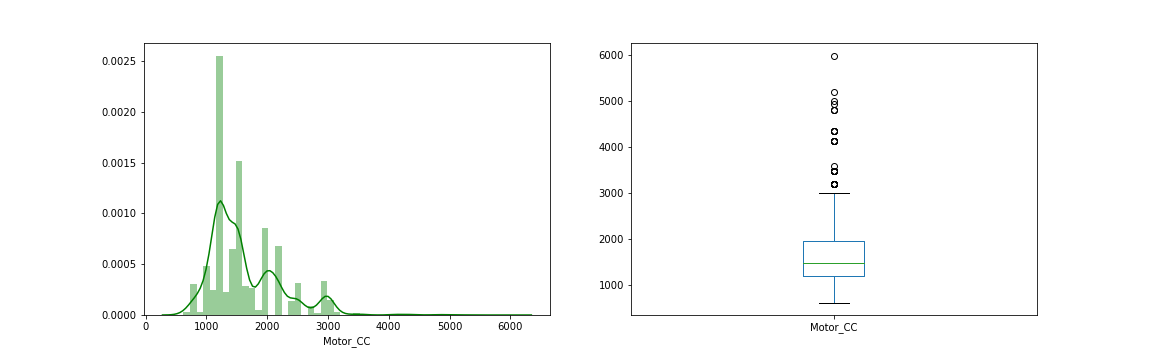
\includegraphics[width=\textwidth]{../notebooks/figures/motor_dis.png}
\caption{Distribución Motor CC}
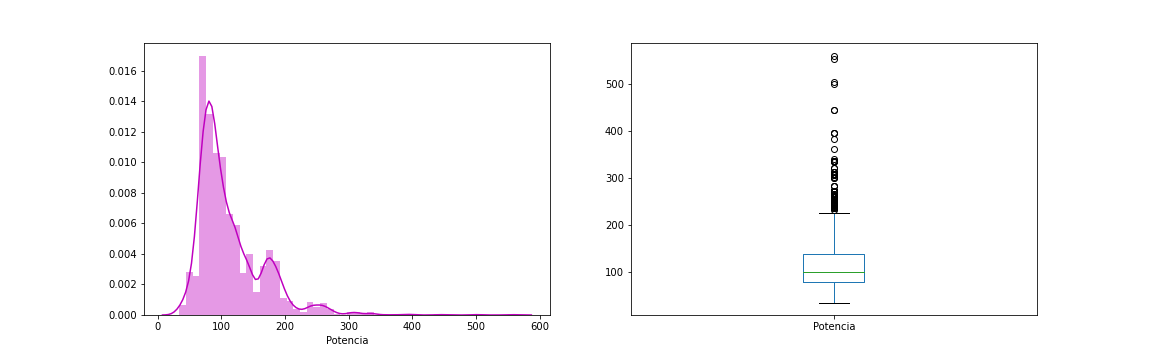
\includegraphics[width=\textwidth]{../notebooks/figures/potencia_dis.png}
\caption{Distribución Potencia}
\label{fig:dis_atributos}
\end{figure}

Como en nuestro histograma inicial, se aprecia la presencia de outliers, por ejemplo en el caso de nuestro atributo \textbf{kilómetros} y asimetría en las distribuciones (\textit{skewed data}), también en nuestro atributo consumo, hay valores de 0, lo cuál creemos que no es posible que haya coches que consuman 0 litros por kilómetro.

Vamos a crear otro atributo llamado \textbf{Company} donde de nuestro atributo \textbf{Nombre} extraeremos la marca del coche (nos quedamos con la primera palabra del nombre que corresponde a la marca del coche), visualizamos la relación entre la marca y el precio en la figura [\ref{fig:eda_marca_precio}] y la distribución de valores de marcas en la figura [\ref{fig:eda_marca}].

\begin{figure}[H]
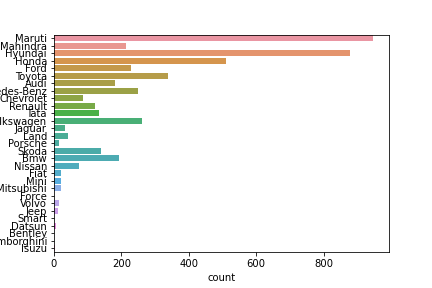
\includegraphics[width=\textwidth]{../notebooks/figures/company.png}
\caption{Marca}
\label{fig:eda_marca}
\end{figure}

En la creación de la nueva columna Company, cuando separabamos los nombres nos hemos encontrado con algunas irregularidades, por ejemplo la marca Isuzu, estaba tanto en mayúscula como en minúscula, esto lo hemos solucionado con el método title() de python, donde hemos unificado estos valores pasándolos a la forma de un String con la primera letra mayúscula, después de esta aclaración, en la figura [\ref{fig:eda_marca_precio}] vemos que la influencia de la marca en el precio tiene sentido, ya que marcas de gama baja suelen valer menos por ejemplo, fiat, comparado con marcas de coches de lujo como por ejemplo, Lamborghini.

\begin{lstlisting}
part = car_train['Nombre'].astype(str).str.partition()
car_train['Company'] = part[0].str.title()
#car_train['Car_name'] = part[2]
\end{lstlisting}

\begin{figure}[H]
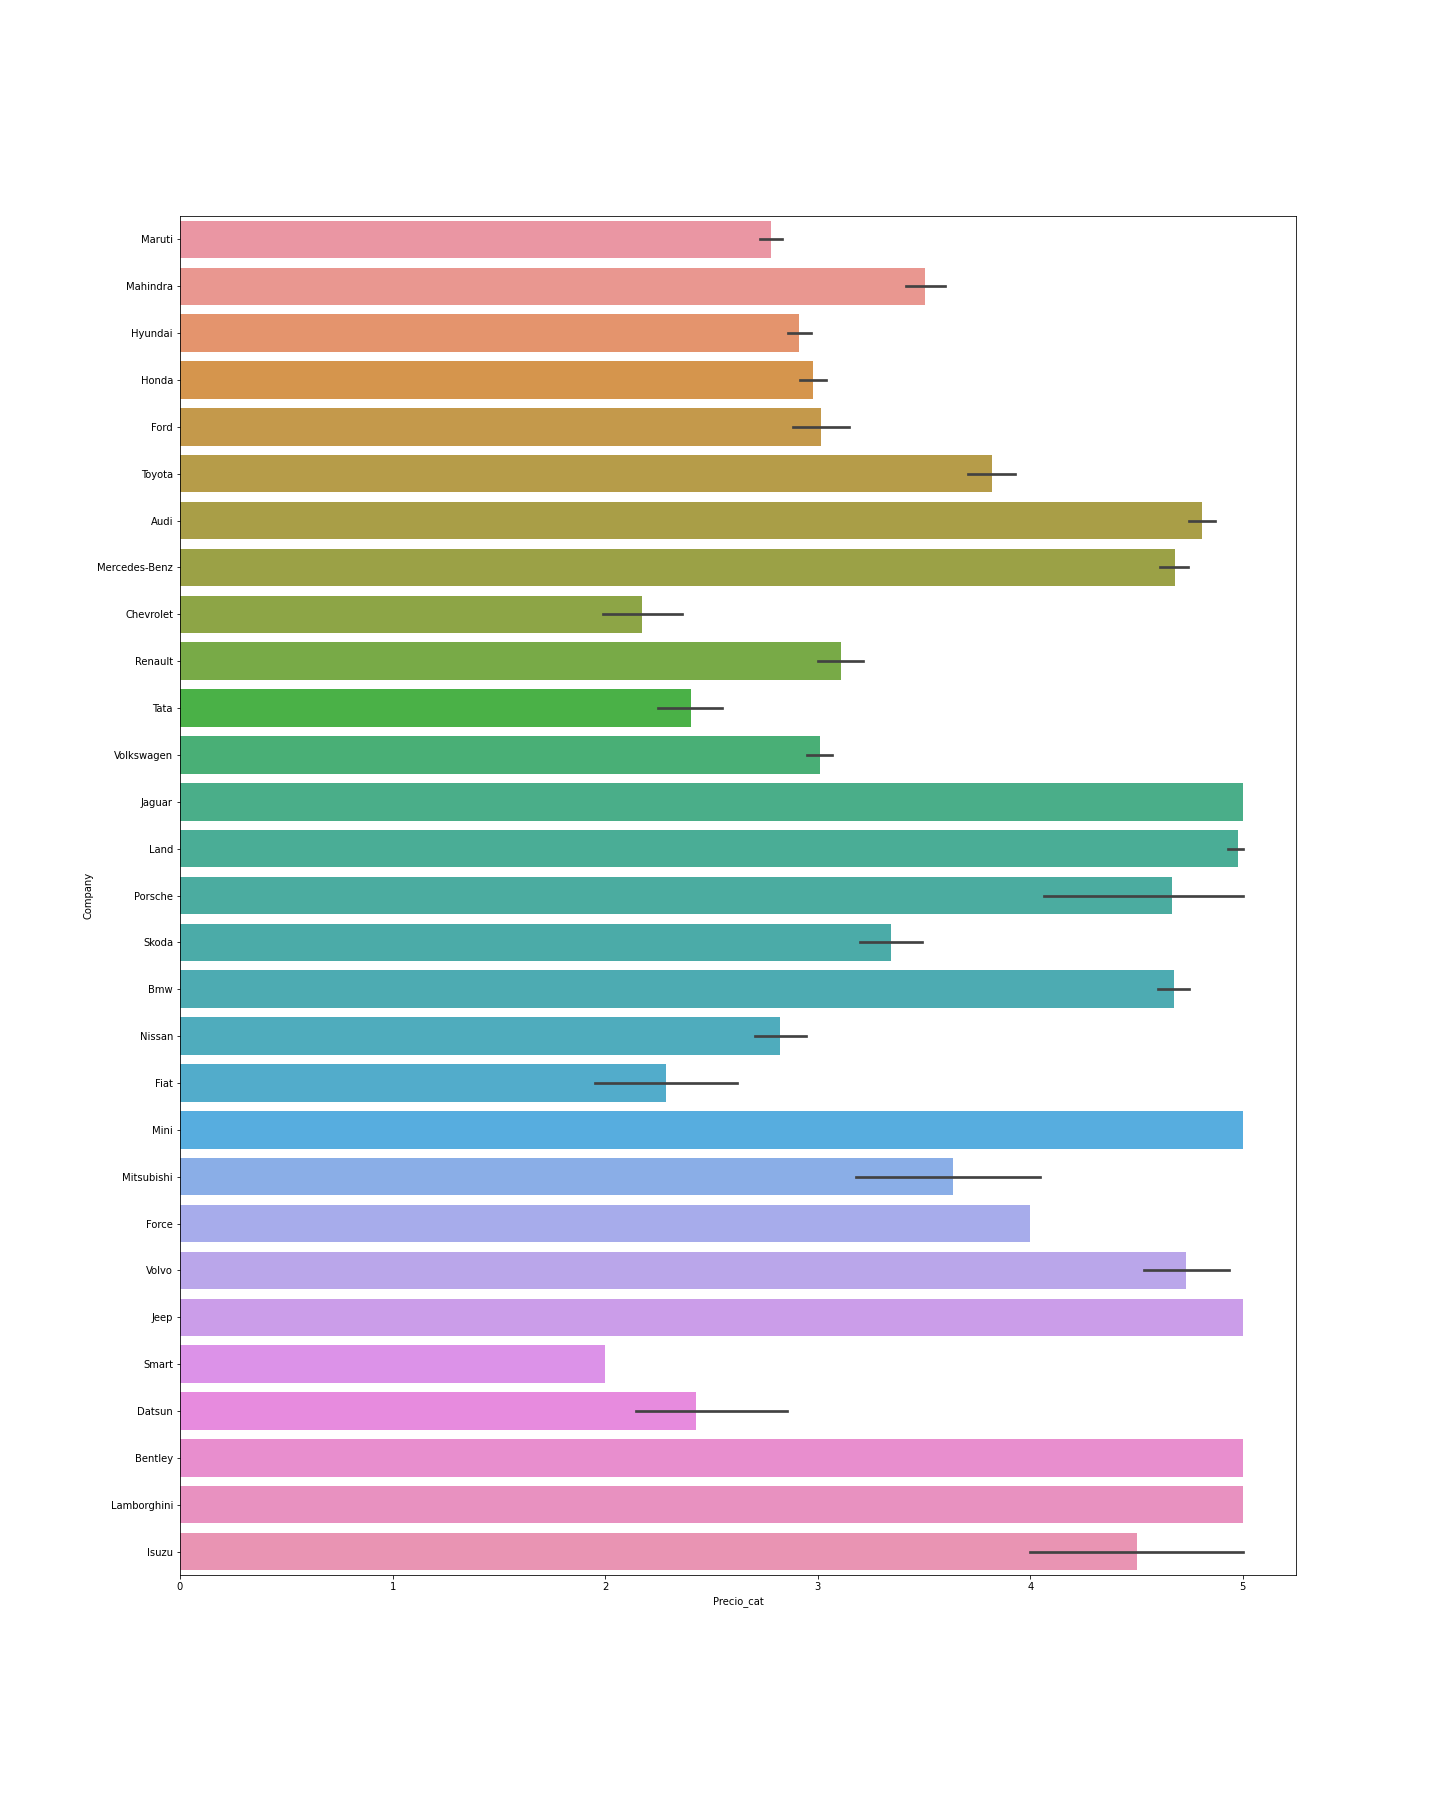
\includegraphics[width=\textwidth]{../notebooks/figures/company_precio_cat.png}
\caption{Marca vs Precio\_cat}
\label{fig:eda_marca_precio}
\end{figure}

Comparamos también entre atributos, por ejemplo entre tipo de marchas y kilómetros en la figura [\ref{fig:tipo_marchas_km}] y entre ciudades y kilometros en la figura [\ref{fig:ciudad_km}]

\begin{figure}[H]
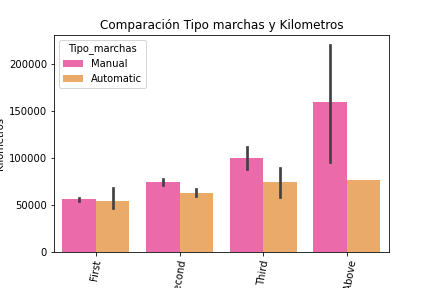
\includegraphics[width=\textwidth]{../notebooks/figures/tipo_marchas_km.png}
\caption{Comparación entre tipo marchas y kilómetros}
\label{fig:tipo_marchas_km}
\end{figure} 


\begin{figure}[H]
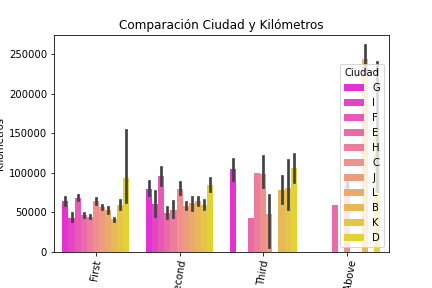
\includegraphics[width=\textwidth]{../notebooks/figures/ciudad_km.png}
\caption{Comparación entre ciudad y kilómetros}
\label{fig:ciudad_km}
\end{figure} 

Añadir heatmap correlación

Algunas conclusiones generales que sacamos de esta visualización es que los atributos característicos tienen un montón de valores únicos, esto puede hacer que realizar un tipo de etiquetado de one hot encoding no sea una buena idea, probaremos con ello igualmente. También hay valores perdidos, trabajaremos con esto probando distintos tipos de preprocesamiento. Finalmente nuestro conjunto esta desbalanceado, realizaremos técnicas de oversample/unversampling para paliar con ello.

\section*{Preprocesamientos}
\addcontentsline{toc}{section}{Preprocesamientos} 

En esta sección vemos distintas maneras que hemos escogido para preprocesar nuestros datos, tratar con valores perdidos, etiquetación, skewed data, outliers y balanceo.

\subsection*{Missing values}
\addcontentsline{toc}{subsection}{Missing values} 

No hay valores duplicados, veamos los valores perdidos de nuestros datasets

\begin{figure}[H]
Train.csv
\begin{multicols}{2}
\begin{tabular}{lrr}
\toprule{} &    percent &  count \\
\midrule Descuento    &  86.324964 &   4160 \\
Potencia     &   3.631459 &    175 \\
Asientos     &   2.199626 &    106 \\
Motor\_CC     &   2.095871 &    101 \\
Consumo      &   1.514837 &     73 \\
Nombre       &   1.494086 &     72 \\
Ciudad       &   1.494086 &     72 \\
Año          &   1.494086 &     72 \\
Kilometros   &   1.494086 &     72 \\
Combustible  &   1.494086 &     72 \\
Tipo\_marchas &   1.494086 &     72 \\
Mano         &   1.494086 &     72 \\
\bottomrule
\end{tabular}



\columnbreak

Test.csv


\begin{tabular}{lrr}
\toprule{} &    percent &  count \\
\midrule Descuento &  86.626402 &   1004 \\
\bottomrule
\end{tabular}
\end{multicols}
\caption{Missing values}
\end{figure}

Debido al porcentaje de valores nulos en nuestro atributo de descuento, siempre vamos a proceder a eliminar esa columna directamente ya que personalmente opino que no sale a cuenta intentar rellenarla  ya que no deja de ser una estimación que por tanto arrastra un error asi que al ser un número tan elevado la descartamos.

Respecto a lo restante, existen un gran número de procedimientos para el tratamiento de valores perdidos, nosotros siempre elegiremos entre eliminar muestras o variables que tienen datos faltantes. (Hay que tener cuidado y garantizar que las variables descartadas no proporcionan información relevante) o sustituir los valores perdidos por estimaciones, por la media si las variables son numéricas (por ejemplo, Kilómetros) o por la moda si las variables son categóricas (Nombre, Mano etc...). 

Antes de aplicar cualquier procedimiento sobre unos datos hay que analizar
la naturaleza de los datos perdidos si los hubiere. Si su origen no fuera
aleatorio, los valores perdidos no pueden ser ignorados. Una vez se sabe que son de origen aleatorio, se debe decidir si eliminarlos o sustituirlos por valores concretos según las técnicas anteriores. Si se tiene un tamaño suficientemente grande de muestras, siempre es preferible
eliminarlos ya que sustituirlos no deja de ser una estimación que por tanto arrastra un error.
Aparte de descartar siempre la columna \textbf{Descuento}, en nuestro caso probaremos siempre tres opciones. 

\begin{itemize}
	\item Eliminar directamente todos los valores nulos
	\item Rellenar los valores nulos con la moda si los atributos son categóricos o con la media sin son numéricos
	\item Crear un nuevo atributo llamado \textbf{Company} como hemos comentado en la parte de visualizacion, y sustituir el valor perdido por la moda de este mismo atributo pero de esa marca. El código sería el siguiente:\\
	\\
	\begin{lstlisting}
	#train.loc[train['brand_name'] == 'Maruti']['Asientos'].mode()[0]
def fill_na_with_mode(ds, brandname, column):
    if ds.loc[ds['Company'] == brandname][column].isnull().any() == False:
        fill_value = ds.loc[ds['Company'] == brandname][column].mode()[0]
        condit = ((ds['Company'] == brandname) & (ds[column].isnull()))
        ds.loc[condit, column] = ds.loc[condit,column].fillna(fill_value)
	\end{lstlisting}
	
	Por ejemplo, si estamos recorriendo los valores perdidos de nuestro atributo \textbf{Asientos}, sustituimos el valor perdido por la moda de Asientos de la marca que corresponda al valor perdido de Asientos. Si no hay siquiera nombre de compañia, no lo hacemos e igualmente luego eliminamos los valores perdidos restantes.
\end{itemize}

\subsection*{Etiquetado}
\addcontentsline{toc}{subsection}{Etiquetado}

Como hemos comentado en la parte de visualización, debido a la gran cantidad de valores únicos de nuestros atributos puede que realizar etiquetados one-hot empeore algunos de nuestros algoritmos, al realizar one hot encoding sobre una variable categórica, estamos induciendo escasez en el conjunto de datos, lo cual no es deseable.
Desde el punto de vista del algoritmo de división, todas las variables ficticias son independientes. Si el árbol decide realizar una división en una de las variables ficticias, la ganancia por división es muy marginal. Como resultado, es muy poco probable que el árbol seleccione una de las variables ficticias más cercanas a la raíz. Para verificar esto, en nuestros modelos que utilicen árboles de decisión veremos la importancia de las características para los modelos y veremos que características destacan. Para realizar un correcto etiquetado utilizando Labels utilizaremos el ejemplo enseñado en los seminarios con los ficheros originales de los datos para el conjunto de train y de test, para probar distintos etiquetamiento one-hot utilizaremos el método \textit{get\_dummies} de pandas. \cite{getdummies}, en la tabla final en la columna de preprocesado comentaremos que variables han sido etiquetadas y como pero nos moveremos entre estos dos tipos de etiquetado. Cabe comentar que cuando realizamos one-hot encoding sobre el conjunto de train y sobre el conjunto de test, puede darse la situacion de que algunas columnas no coincidan, por ejemplo si se diera el caso que como hemos comentado antes, crear una columna con marcas de vehículos y aplicar one-hot encoding sobre la misma, el conjunto de test no tiene porque tener las mismas columnas que el conjunto de train, luego esto daría un error de dimensión, para ello si se diera el caso rellenamos el conjunto de test con columnas faltantes vacías con 0s, adjuntamos una parte del script para ello.

\begin{lstlisting}
# Get missing columns in the training test
missing_cols = set( train.columns ) - set( test.columns )
# Add a missing column in test set with default value equal to 0
for c in missing_cols:
    test[c] = 0
# Ensure the order of column in the test set is in the same order than in train set
test = test[train.columns]
\end{lstlisting}

\subsection*{Escalado}
\addcontentsline{toc}{subsection}{Escalado}
En la práctica, siempre viene bien escalar los datos (Estandarizar características eliminando la media y escalando a la varianza de la unidad), en nuestro caso después de varias pruebas, aunque hacemos uso de modelos basados en distancias, no son ni de lejos los que mejores resultados proporcionan, así que en nuestro caso tratar con el escalado de los datos no será importante ya que no influira en nuestros mejores resultados. Los modelos basados en distancias mejoran drásticamente mientras que para otros es irrelevante. Respecto a normalizar, probando un par de veces vemos que no beneficia nada a nuestro problema asi que no normalizaremos nuestros datos. En conclusión, aplicaremos escalado ya que nuestros modelos basados en distancia se benefician, y los que no (que también son los que mejores resultados nos aportan) son indiferentes ante este escalado asi que digamos que escalar no "molesta". No normalizaremos porque solo perjudica.

\subsection*{Skewed data y outliers}
\addcontentsline{toc}{subsection}{Skewed data y outliers}

Como hemos visto en la parte de visualización, tenemos skewed data y outliers en nuestros atributos, vamos a tratar los outliers de algunos de nuestros atributos, vamos a documentar un ejemplo de lo que sería un preprocesamiento completo de outliers y skewed data, aunque estos pueden realizarse individualmente y el resultado e imágenes en cuyo caso serán distintos, se dirá si se ha tenido en cuenta o no en la tabla final este tipo de preprocesamiento.

En la figura [\ref{fig:outliers_data}] mostramos 4 boxplots donde se aprecia claramente los outliers de nuestro conjunto, cabe comentar en el atributo consumo los valores 0.0, como ya hemos comentado en la parte de visualización, dudamos entre transformar estos atributos a valores nulos o eliminarlos directamente, en este caso vamos a proceder a eliminarlos. y a quedarnos con los datos más centrados.

\begin{figure}[H]
\begin{multicols}{2}
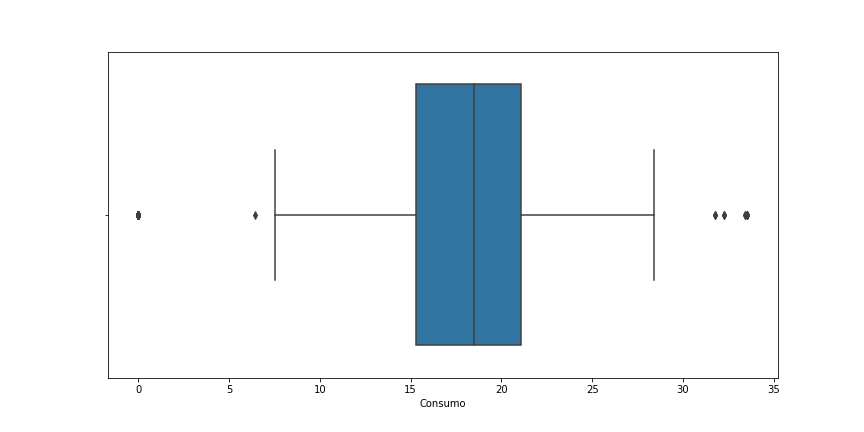
\includegraphics[width=8cm]{../notebooks/figures/outlier_Consumo.png}
\caption{Outliers consumo}
\columnbreak
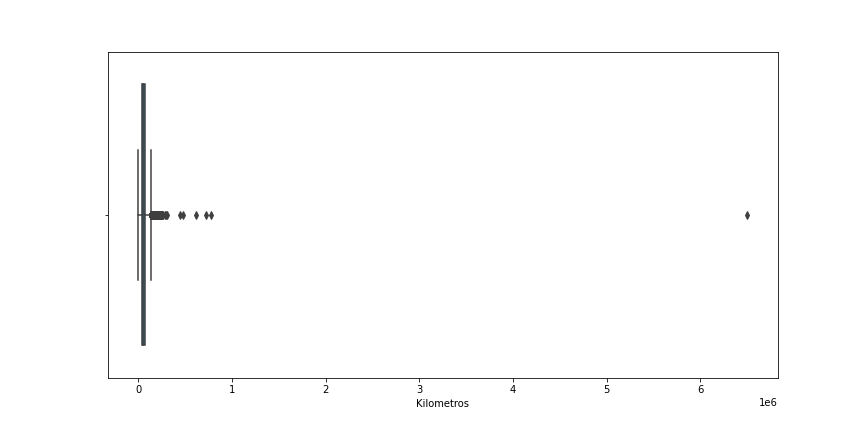
\includegraphics[width=8cm]{../notebooks/figures/outlier_Kilometros.png}
\caption{Outliers Kilometros}
\end{multicols}
\begin{multicols}{2}
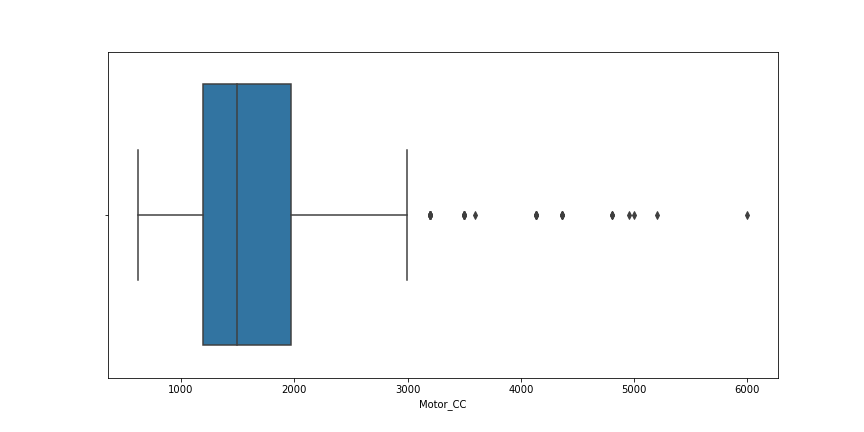
\includegraphics[width=8cm]{../notebooks/figures/outlier_Motor_CC.png}
\caption{Outliers Motor\_CC}
\columnbreak
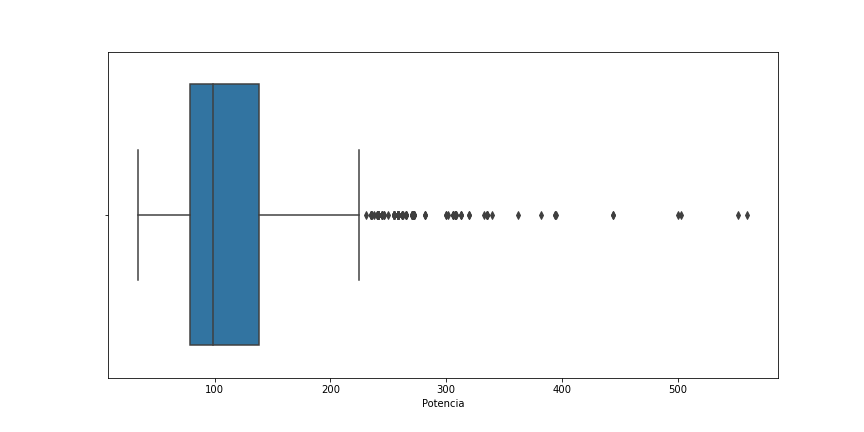
\includegraphics[width=8cm]{../notebooks/figures/outlier_Potencia.png}
\caption{Outliers Potencia}
\end{multicols}
\caption{Outliers}
\label{fig:outliers_data}
\end{figure} 

Podemos usar la funcion \textit{quantile} de python para ver los quantiles de los extremos, en nuestro caso son:

\begin{lstlisting}
Kilometros
max threshold : 451370.00000002445
min threshold : 1000.0
Potencia
max threshold : 456.93420000002664
min threshold : 34.2
Consumo
max threshold : 33.44
min threshold : 0.0
Motor_CC
max threshold : 4959.918000000034
min threshold : 624.0
\end{lstlisting}

Vamos a reducir estos outliers, por ejemplo acotandolo por estos valores:

\begin{lstlisting}
train=train[train['Kilometros'] < 262000]             
train=train[train['Consumo'] > 0.0]        
train=train[train['Potencia'] <= 530]
train=train[train['Motor_CC'] <= 5900 ]
\end{lstlisting}

Después de nuestra transformación los datos quedarían como en la figura [\ref{fig:no_outliers_data}]

\begin{figure}[H]
\begin{multicols}{2}
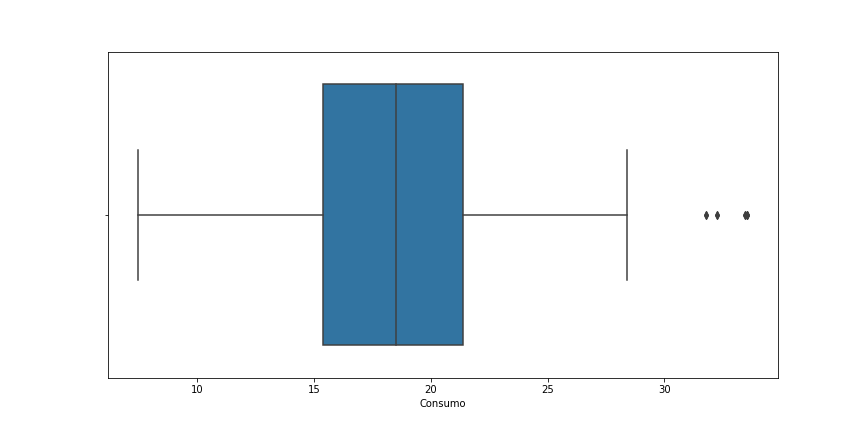
\includegraphics[width=8cm]{../notebooks/figures/no_outlier_Consumo.png}
\caption{No outliers consumo}
\columnbreak
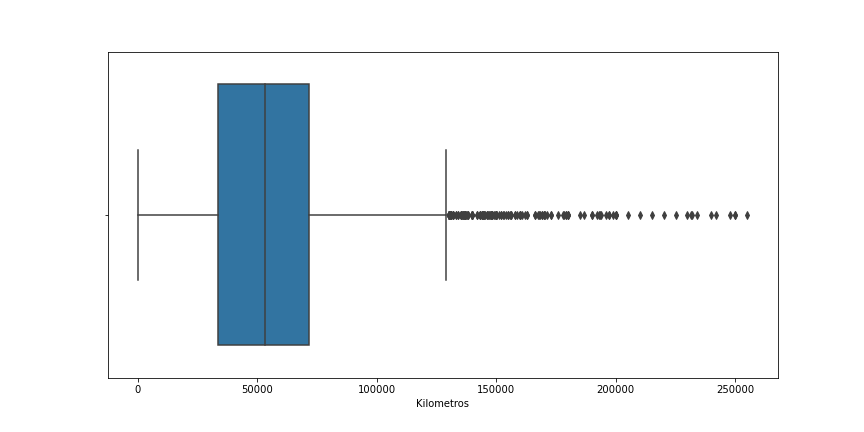
\includegraphics[width=8cm]{../notebooks/figures/no_outlier_Kilometros.png}
\caption{No outliers Kilometros}
\end{multicols}
\begin{multicols}{2}
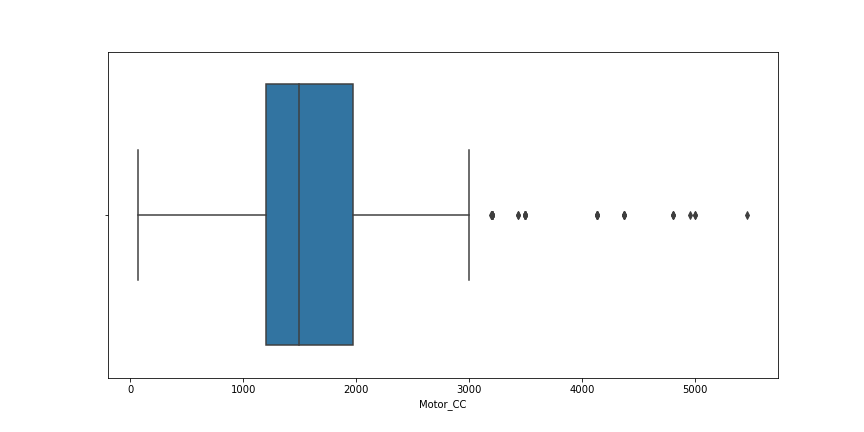
\includegraphics[width=8cm]{../notebooks/figures/no_outlier_Motor_CC.png}
\caption{No outliers Motor\_CC}
\columnbreak
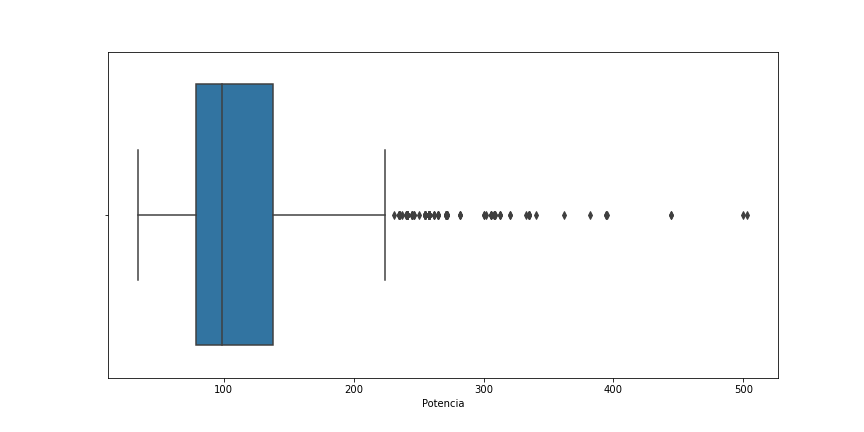
\includegraphics[width=8cm]{../notebooks/figures/no_outlier_Potencia.png}
\caption{No outliers Potencia}
\end{multicols}
\caption{No outliers}
\label{fig:no_outliers_data}
\end{figure} 



Por lo tanto, en los datos asimétricos,los outliers del skewed data pueden actuar como un valor atípico para el modelo estadístico y sabemos que los valores atípicos afectan negativamente el rendimiento del modelo, (especialmente los modelos basados en regresión). Hay modelos estadísticos que son robustos a valores atípicos como los modelos basados en árboles, pero limitarán la posibilidad de probar otros modelos. Por lo tanto, es necesario transformar los datos asimétricos para que se acerquen lo suficiente a una distribución gaussiana o distribución normal. 


Por otro lado, en nuestros atributos, un dato se denomina skewed (\textit{sesgado}) cuando la curva aparece distorsionada o sesgada hacia la izquierda o hacia la derecha, en una distribución estadística. En nuestro caso profundizemos en nuestros atributos Kilometros, Potencia, Consumo y Motor\_CC. Usamos la función skew \cite{skew} de la librería pandas para comprobar la asimetría de nuestros datos, un valor de asimetría de 0 en la salida denota una distribución simétrica de valores en la fila 1, un valor de asimetría negativo en la salida indica una asimetría en la distribución correspondiente a la izquierda y la cola es más grande hacia el lado izquierdo de la distribución mientras que un valor de asimetría positivo en la salida indica una asimetría en la distribución correspondiente a derecha y la cola es más grande hacia el lado derecho de la distribución. Adjuntamos una tabla con lo comentado:

\begin{center}
\begin{tabular}{lr}
\toprule{} &  skewness \\
\midrule Potencia   &  1.851863 \\
Motor\_CC   &  1.397533 \\
Kilometros &  1.369657 \\
Consumo    &  0.177833 \\
\bottomrule
\end{tabular}
\end{center}

En una distribución normal, el gráfico tiene simetría, lo que significa que hay tantos valores de datos en el lado izquierdo de la mediana como en el lado derecho. En la figura [\ref{fig:skewed_data}] vemos la distribución de nuestros datos.

\begin{figure}[H]
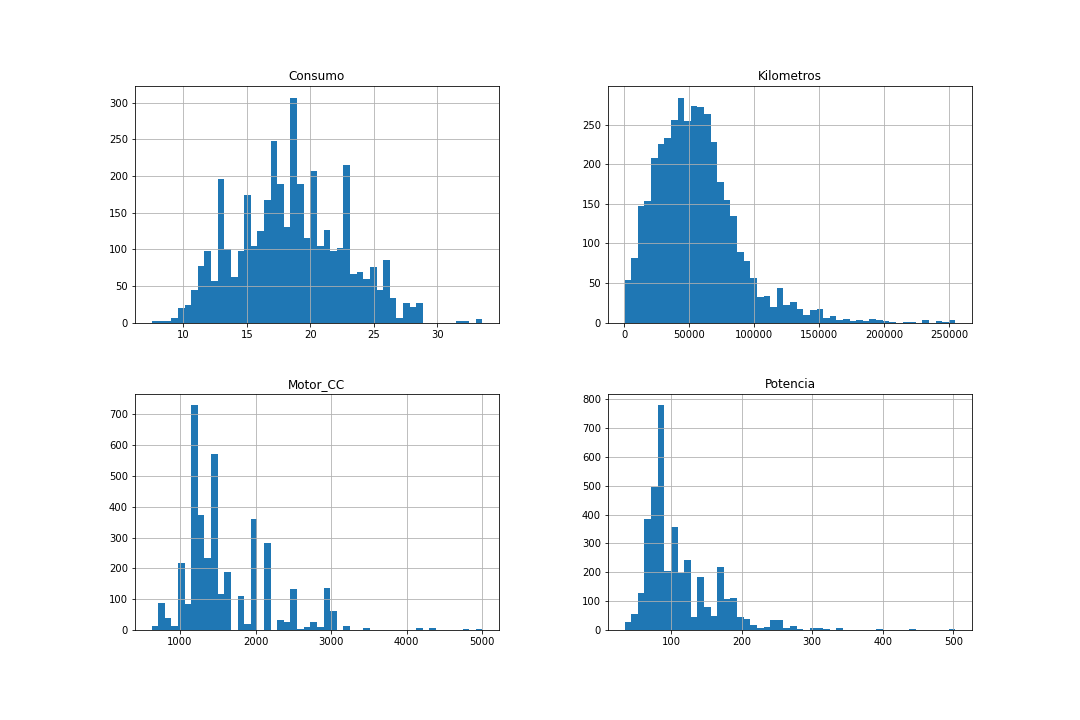
\includegraphics[width=\textwidth]{../notebooks/figures/skewed_data.png}
\caption{Skewed data}
\label{fig:skewed_data}
\end{figure} 

Aplicamos logarítmos para tratar con estos datos sesgados en la figura [\ref{fig:no_skewed_data}] vemos el resultado de nuestros datos después de haber aplicado técnicas logarítmicas

\begin{figure}[H]
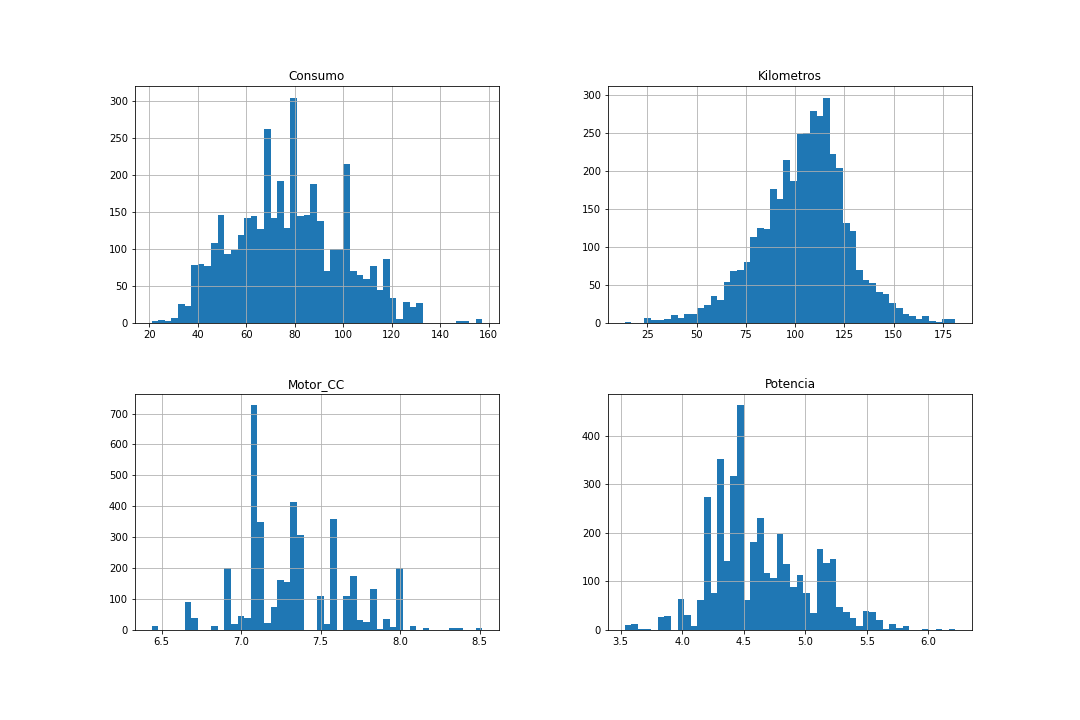
\includegraphics[width=\textwidth]{../notebooks/figures/no_skewed_data.png}
\caption{Skewed data}
\label{fig:no_skewed_data}
\end{figure} 

Mostramos una tabla con los datos transformados para medir el nivel de skew.
\begin{center}
\begin{tabular}{lr}
\toprule{} &  skewness \\
\midrule
Potencia   &  0.540517 \\
Motor\_CC   &  0.303247\\
Consumo    &  0.186635 \\
Kilometros & -0.275876 \\
\bottomrule
\end{tabular}
\end{center}


\subsection*{Balanceado}
\addcontentsline{toc}{subsection}{Balanceado}
Cuando procedemos a dividir nuestro conjunto de entrenamiento entre la variable a predecir y el resto de atributos, nos encontramos con que nuestra variable a predecir, \textbf{Precio\_cat} esta muy desbalanceada, hay siempre un valor entre los 5 a predecir que en mucha más cantidad que el resto, si una clase está sobrerepresentada frente al resto, el modelo tendrá mucha tendencia a elegirlo. Esto puede ser problemático o no, si los datos finales a predecir mantienen el mismo no-balanceamiento, pero si no fuese el caso sí podría dar problemas, mientras que si una clase aparece poco en las muestras respecto al resto el modelo puede tener tendencia a despreciar dicha clase ya que le afecta poco a sus medidas, llegando incluso a ignorarla en casos extremos. Esto se produce independientemente de si dicho no-balanceamiento aparece también en los datos finales sobre los que se vaya a predecir. La gravedad depende del nivel de desbalanceamiento y de si el conjunto de datos a predecir mantiene el balanceamiento o no, pero en cualquier caso puede ser problemático, y es recomendable tratarlo.

Dependendiendo de las características puede ser más conveniente uno que otro: undersampling, y oversampling. En nuestro caso probar con ambas técnicas llegados a la conclusión de que undersampling no es adecuado para nuestro caso, ya que elimina ejemplos de la clase mayoritaria y puede resultar en la pérdida de información invaluable para los modelos. Asi que nos centramos principalmente en oversampling, de todos los distintos preprocesamientos el que más ganancia nos ha aportado en una mejor puntuación del modelo es este tipo de preprocesamiento en la variable a predecir, al principio comenzamos con el que se ha dado en clase de prácticas, Synthetic Minority Oversampling Technique (\textbf{SMOTE}, sintetiza nuevos ejemplos para la clase minoritaria), pero luego empezamos a utilizar \textbf{RandomOverSampling} (duplica ejemplos de la clase minoritaria en el conjunto de datos de entrenamiento, tarde nos dimos cuenta que esto puede resultar en un "overfitting" para algunos modelos) ya que nos proporcionaba mejores resultados. Se describirá en la tabla que tipo de balanceo se ha aplicado.

\section*{Algoritmos}
\addcontentsline{toc}{section}{Algoritmos}  

Aunque hemos usado gran cantidad de algorítmos de clasificación (SVM, KNeighbors, Extra Tree etc...), al final nos centramos solo en 3 de ellos ya que son los que mejores resultados nos proporcionan en nuestro conjunto train, vamos a comentarlos. Respecto a los preprocesamientos realizados para cada algoritmo, se escribirá explícitamente en la tabla, aunque el que más mejora ha resultado ser el trato con el balanceo, respecto a por ejemplo valores perdidos, escalado y demás, la mejora de esto es mínima, menos de 3\% en todos los casos. Como hemos comentado en la parte de escalado, al ser algoritmos que no funcionan por distancia es normal que no influya la escala de los datos, además de ser métodos que funcionan bien aunque nuestro dataset no tengan muchos valores.

\subsection*{Random Forest}
\addcontentsline{toc}{subsection}{Random Forest}

\textbf{Random Forest Classifier}\cite{rfc} es un metaestimador que se ajusta a una serie de clasificadores de árboles de decisión en varias submuestras del conjunto de datos y utiliza promedios para mejorar la precisión predictiva y controlar el sobreajuste. Funciona bien en la mayoría de problemas, y en este no es una excepción, En nuestro caso aunque proporciona buenos resultados el problema es su overfitting muy rápido, por ello en algunas de nuestras subidas de ficheros a Kaggle se ha obtenido puntuaciones pésimas (alrededor de 0.2).

Para evitar un sobre ajuste excesivo lo que hemos intentado hacer es reducir el parámetro \textit{max\_depth} y optimizar parámetros de ajuste que controlen la cantidad de características que se eligen al azar para hacer crecer cada árbol a partir de los datos de arranque. La función que hemos utilizado para hacer tuning de nuestro algoritmo es la siguiente:\\
\\

\begin{lstlisting}
def best_tree(X_train, y_train):
    #Randomized Search CV

    # Number of trees in random forest
    n_estimators = [int(x) for x in np.linspace(start = 100, stop = 1200, num = 12)]
    # Number of features to consider at every split
    max_features = ['auto', 'sqrt']
    # Maximum number of levels in tree 3-10 to deal with overfitting
    max_depth = [3, 4, 5, 6, 7, 8, 9]
    # Minimum number of samples required to split a node
    min_samples_split = [2, 5, 10, 15, 100]
    # Minimum number of samples required at each leaf node
    min_samples_leaf = [1, 2, 5, 10]
    
    # Create the random grid
    random_grid = {'n_estimators': n_estimators,
                   'max_features': max_features,
                   'max_depth': max_depth,
                   'min_samples_split': min_samples_split,
                   'min_samples_leaf': min_samples_leaf}
    
    # search across different combinations
    rf_random = RandomizedSearchCV(estimator = RandomForestClassifier(), 
                                   param_distributions = random_grid, 
                                   scoring=scoring, 
                                   n_iter = 15, cv = 5, verbose=2, random_state=42, n_jobs = 1)
    
    rf_random.fit(X_train,y_train)
    
    return rf_random
\end{lstlisting}

Hemos elegido randomized search en vez de grid search ya que exploran exactamente el mismo espacio de parámetros y el resultado en la configuración de los parámetros es bastante similar, mientras que el tiempo de ejecución para la búsqueda aleatoria es drásticamente menor. \cite{random-grid}

Después de controlar el overfitting haciendo tuning de los parámetros mostrados anteriormente, se consiguen peores puntuaciones respecto a nuestro conjunto de train (lo cuál es normal, pero antes obteniamos puntuaciones perfectas lo que nos indicaba un claro overfitting) pero obtenemos mejores puntuaciones en nuestro conjunto de test. Se escribirá en la tabla cuales han sido los parámetros elegidos. Otra cosa buena del random forest es que podemos ver que características han tenido más importancia, por ejemplo en la figura [\ref{fig:rfc_features}] vemos un ejemplo de esto. Respecto a los preprocesamientos, como hemos comentado al inicio de esta sección, no se ha notado mucha mejoría excepto cuando tratamos con el desbalanceo.

\begin{figure}[H]
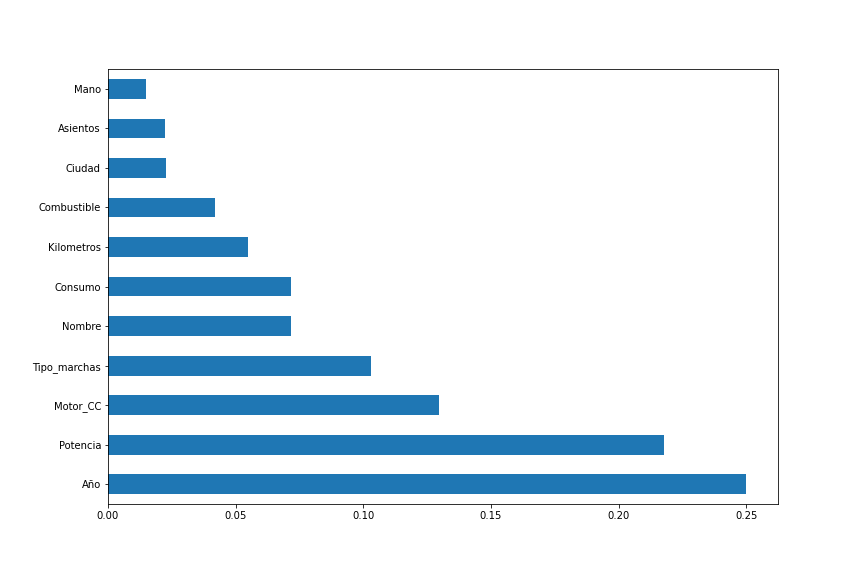
\includegraphics[width=\textwidth]{../notebooks/figures/feature_importances_rfc_1.png}
\caption{Features importance}
\label{fig:rfc_features}
\end{figure} 

También cabe decir que aunque no es el modelo que nos proporciona mejores resultados, sin duda es el que más rápido funciona.

\subsection*{XGBoost}
\addcontentsline{toc}{subsection}{XGBoost}

El algoritmo \textbf{XGBoost}\cite{xgboost} es eficaz para una amplia gama de problemas de modelos predictivos de clasificación.

Es una implementación eficiente del algoritmo de stochastic gradient boosting y ofrece una gama de hiperparámetros que brindan un control detallado sobre el procedimiento de entrenamiento del modelo. Aunque el algoritmo funciona bien en general, incluso en conjuntos de datos de clasificación desequilibrados, ofrece una forma de ajustar el algoritmo de entrenamiento para prestar más atención a la clasificación errónea de la clase minoritaria para conjuntos de datos con una distribución de clases sesgada. Está basado en un Random Forest ponderando a los individuos que se clasificaron mal en árboles anteriores. Al igual que en el caso de random forest classifier, XGBoost (y otros algoritmos de gradient boosting) tiene una serie de parámetros que se pueden ajustar para evitar un sobreajuste. La documentación está bastante bien respecto a estos parámetros \cite{xgboost-tuning}, nuestra función de tuning es la siguiente:\\
\\

\begin{lstlisting}
def best_xgboost(X_train, X_test, y_train, y_test):
    
    param_dist = {'n_estimators': [int(x) for x in np.linspace(start = 100, stop = 1000, num = 12)],
# the learning rate of our GBM (i.e. how much we update our prediction with each successive tree); eta.
# Lower values avoid over-fitting.                  
              'learning_rate': [0.01, 0.05, 0.1, 0.15, 0.2, 0.3, 0.4, 0.5],
              'subsample': [0.3, 0.4, 0.5, 0.6, 0.7, 0.8, 0.9, 1.],
# the maximum depth of a tree; max_depth. Lower values avoid over-fitting                  
              'max_depth': [3, 4, 5, 6, 7, 8],
# the ratio of features used (i.e. columns used); colsample_bytree. Lower ratios avoid over-fitting.
              'colsample_bytree': [0.5, 0.6, 0.7, 0.8, 0.9, 1.],
# the minimum sum of instance weight needed in a leaf, in certain applications this relates directly to 
# the minimum number of instances needed in a node; min_child_weight. Larger values avoid over-fitting.                  
              'min_child_weight': [1, 5, 15, 20, 50]
             }
    
    print(param_dist)

    xgboost_random = RandomizedSearchCV(estimator = XGBClassifier(), 
                               param_distributions = param_dist, 
                               scoring=scoring, 
                               n_iter = 15, cv = 5, verbose=2, random_state=42, n_jobs = 1)
    
    xgboost_random.fit(X_train, y_train, eval_metric = "mlogloss", eval_set = [(X_test, y_test)])
    
    return xgboost_random
\end{lstlisting}

Destacamos también el parámetro \textit{subsample} Proporción de submuestras de las instancias de formación. Establecerlo en 0.5 significa que XGBoost muestreará al azar la mitad de los datos de entrenamiento antes de cultivar árboles. y esto evitará el sobreajuste. Se escribirá en la tabla el conjunto de parámetros utilizados en el algoritmo para la predicción.

El modelo XGBoost puede evaluar e informar sobre el rendimiento en un conjunto de prueba para el modelo durante el entrenamiento.

Admite esta capacidad especificando tanto un conjunto de datos de prueba como una métrica de evaluación en la llamada a model.fit () al entrenar el modelo y especificar una salida detallada.

En nuestro caso hemos elegido informar sobre la tasa de error de clasificación multiclase \textit{mlogloss} en un conjunto de prueba independiente (eval\_set) mientras entrenamos el modelo XGBoost. Produce mejores resultados que el random forest aunque en comparación al tiempo es muchísimo más lento.

\subsection*{Catboost}
\addcontentsline{toc}{subsection}{Catboost}

\textbf{CatBoost} \cite{catboost} es una biblioteca de software open-source desarrollada por Yandex. Proporciona un framework gradient boosting que intenta resolver las características categóricas utilizando una alternativa impulsada por permutación en comparación con un algoritmo clásico. Mientras que XGBoost fue el algoritmo más competitivo y preciso en Kaggle la mayor parte del tiempo, ahora está de moda un nuevo líder llamado \textbf{CatBoost}. En su documentación, incluyen referencias y ejemplos de GitHub, noticias, evaluaciones comparativas, comentarios, contactos, tutorial e instalación. Si está utilizando XGBoost, LightGBM o H2O, la documentación de CatBoost ha realizado una evaluación comparativa y ha demostrado que son los mejores con resultados ajustados y predeterminados. Por supuesto, si tiene variables más categóricas, CatBoost es el camino a seguir. Esta biblioteca permite algunas visualizaciones impresionantes, incluido el proceso de prueba y entrenamiento del modelo y una impresión de la importancia de las características, por nombrar algunas. 
Al contrario que en la mayoría de los algoritmos, en el caso de catboost \textbf{no hay que realizar one-hot encoding sobre los datos durante el preprocesamiento} \cite{catboost-onehot}, ya que esto afecta tanto a la velocidad del entrenamiento como a la calidad resultante. Por el contrario, hay un parámetro \textit{one\_hot\_max\_size} que podemos usar para cambiar el número máximo de valores únicos de características categóricas para aplicar la codificación one-hot. Lo que significa que CatBoost no requiere la conversión del conjunto de datos a ningún formato específico como XGBoost y LightGBM. También cabe decir que \textbf{Catboost} soporta la opción de entrenar el modelo utilizando la GPU, en nuestro caso esto no será posible ya que no contamos con un ordenador que tenga una GPU.

De igual manera a nuestros algoritmos anteriores, mostramos la función que hemos elegido para hacer tuning de nuestro algoritmo, al contrario que en los casos anteriores, aquí usamos funciones exclusivas de la librería de catboost:\\

\begin{lstlisting}
def best_catboost(X_train, y_train):
    
    grid = {
        'iterations': [800, 1000, 1200], 
        'learning_rate': [0.03, 0.06, 0.1],
        'random_strength': [0.03, 0.06, 0.1],
        'depth': [4, 5, 6, 7, 8, 9, 10],
        'one_hot_max_size': [2,3,4,5,6,7,8],
        'od_type': ['IncToDec', 'Iter']}
    
    model = CatBoostClassifier(loss_function='MultiClass', eval_metric='Accuracy', leaf_estimation_method='Newton')
    
    randomized_search_result = model.randomized_search(grid,
                                                       X=X_train,
                                                       y=y_train,
                                                       cv=5, n_iter=15,plot=True)    
    return randomized_search_result
\end{lstlisting}

\textbf{Catboost} cuenta con detectores de sobreajuste, \cite{catboost-overfit}, si se produce un sobreajuste, CatBoost puede detener el entrenamiento antes de lo que dicten los parámetros de entrenamiento. Por ejemplo, se puede detener antes de que se construya el número especificado de árboles. El método de detección de sobreajuste se establece en el parámetro \textit{od\_type}. Mantenemos siempre los parámetros de \textit{loss\_function} y \textit{eval\_metric} a esos valores ya que son los que se aplican a nuestro problema.

Como hemos comentado antes, también podemos ver en una gráfica dinámica como se entrena nuestro modelo en tiempo real según los dos parámetros de evaluación y pérdida, vemos un ejemplo en la figura [\ref{fig:catboost_train}].

\begin{figure}[H]
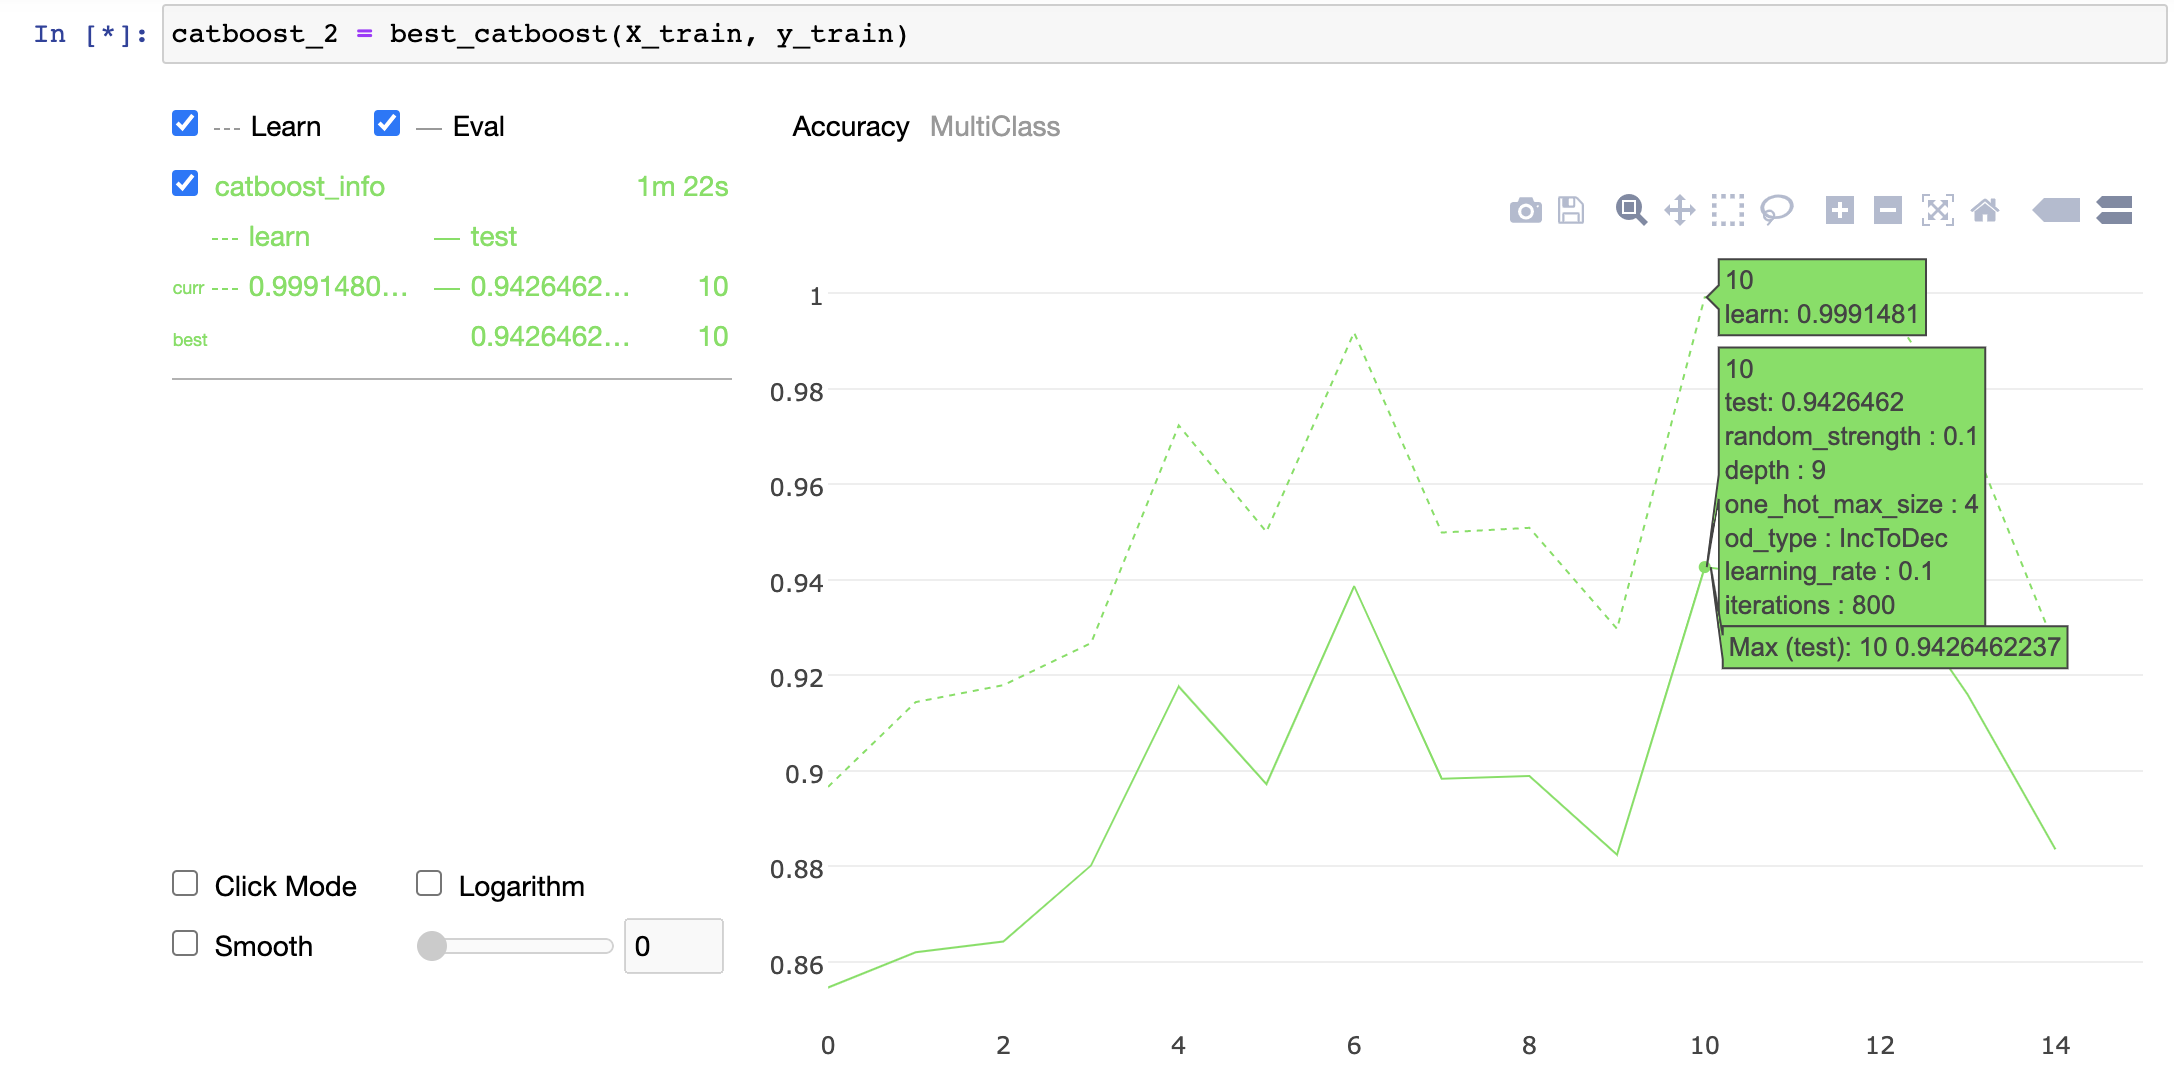
\includegraphics[width=\textwidth]{../notebooks/figures/catboost_train.png}
\caption{Catboost plot train}
\label{fig:catboost_train}
\end{figure} 

Este algoritmo ha sido el que mejores resultados nos ha proporcionado, y el que nos ha dado nuestra mejor puntuación, respecto al tiempo he de decir que tarda bastante si se hace tuning, (y más con la gráfica) aunque más o menos tarda lo mismo que xgboost
\section*{Red Neuronal}
\addcontentsline{toc}{section}{Red Neuronal}  

Dedicamos una sección especial a la propuesta de una red neuronal con Keras \footnote{La red neuronal puede encontrarse en un notebook aparte llamado neural\_network.ipynb}.

Para la creación de la red neuronal, creamos un modelo secuencia \cite{keras-sequential}, a los que se les ha ido añadiendo varias capas densas \cite{keras-dense}, a partir de estos modelos mostramos en varias gráficas la ganancia y perdida para cada uno de los modelos y nos quedamos con el que más nos convenga.

Resumimos nuestro modelo en lo siguiente:

\begin{itemize}
	\item Input Layer: Layer de entrada, creamos una capa densa con el número de inputs, esto depende del número de atributos que tengamos en ese momento y depende del tipo de preprocesado, por ejemplo si simplemente aplicamos etiquetación a todos nuestros atributos tendremos una dimensión de 11 (11 atributos), mientras que si realizamos one hot encoding este número aumentara al tener más columnas.
	\item Hidden Layers: Layers de nodos entre el layer de input y de output, son capas densas que añadimos en el número que queramos, como máximo probaremos 5.
	\item Output Layer: El layer que produce el output, tendra el número de nodos de nuestra variable a predecir, en formato one-hot, en nuestro caso es un valor entre 1-5 que aplicado con one-hot encoding es 5.
\end{itemize}

Para nuestras capas densas, vamos a usar siempre funciones de activación \textit{relu}, excepto en nuestro último layer de output, que usaremos \textit{softmax}, debido a que funciona bien para problemas multiclase como output \cite{softmax}. Softmax asigna probabilidades decimales a cada clase en un problema de varias clases. Esas probabilidades decimales deben sumar 1.0. Esta restricción adicional ayuda a que el entrenamiento converja más rápidamente de lo que lo haría de otra manera. El código de creación de nuestro modelo es el siguiente:\\
\\
\begin{lstlisting}
def create_custom_model(input_dim, output_dim, nodes, n=1, name='model'):
    def create_model():
        # Create model
        model = Sequential(name=name)
        for i in range(n):
            model.add(Dense(nodes, input_dim=input_dim, activation='relu'))
        model.add(Dense(output_dim, activation='softmax'))

        # Compile model
        model.compile(loss='categorical_crossentropy', 
                      optimizer='adam', 
                      metrics=['accuracy'])
        return model
    return create_model
\end{lstlisting}

Respecto a optimizador hemos escogido \textit{Adam} ya que combina las buenas propiedades de Adadelta y RMSprop y, por lo tanto, tiende a funcionar mejor para la mayoría de los problemas y \textit{loss} categorical\_crossentropy ya que es un problema de clasificación multiclase. 

Para la creación de nuestro modelo muchos de los valores de parámetros se han elegido empíricamente, por ejemplo para la elección de nodos de cada uno de nuestros hidden layers, haciendo un poco de investigación vemos que no hay una fórmula objetiva para escogerlos. \cite{nodes-hidden}. En nuestro caso hemos elegido la fórmula $$ N_h =\frac{N_s}{( \alpha*(N_i+N_o))}$$ donde 
\begin{itemize}
	\item $N_i$ número de neuronas de entrada
	\item $N_o$ número de neuronas de output
	\item $N_s$ número de ejemplos del conjunto de entrenamiento
	\item $\alpha$ un factor arbitrario entre 5 y 10 (en nuestro caso hemos escogido 5)
\end{itemize}

\textbf{Haremos un ejemplo de ejecución donde como preprocesado escogemos llenar los valores perdidos numéricos con la media y categóricos con la moda, utilizaremos label encoding para nuestros atributos y para el balanceo utilizamos RandomOverSampling}.\\
\\
\begin{lstlisting}
alpha = 5
nodes = n_samples // (alpha * (n_features + n_classes))
print("Number of nodes:", nodes)
models = [create_custom_model(n_features, n_classes, nodes, i, 'model_{}'.format(i)) 
          for i in range(1, 6)]

for create_model in models:
    create_model().summary()
\end{lstlisting}
\begin{lstlisting}
Number of nodes: 69
_________________________________________________________________
Layer (type)                 Output Shape              Param #   
=================================================================
dense_1 (Dense)              (None, 69)                828       
_________________________________________________________________
dense_2 (Dense)              (None, 5)                 350       
=================================================================
Total params: 1,178
Trainable params: 1,178
Non-trainable params: 0
_________________________________________________________________
_________________________________________________________________
Layer (type)                 Output Shape              Param #   
=================================================================
dense_3 (Dense)              (None, 69)                828       
_________________________________________________________________
dense_4 (Dense)              (None, 69)                4830      
_________________________________________________________________
dense_5 (Dense)              (None, 5)                 350       
=================================================================
Total params: 6,008
Trainable params: 6,008
Non-trainable params: 0
_________________________________________________________________
_________________________________________________________________
Layer (type)                 Output Shape              Param #   
=================================================================
dense_6 (Dense)              (None, 69)                828       
_________________________________________________________________
dense_7 (Dense)              (None, 69)                4830      
_________________________________________________________________
dense_8 (Dense)              (None, 69)                4830      
_________________________________________________________________
dense_9 (Dense)              (None, 5)                 350       
=================================================================
Total params: 10,838
Trainable params: 10,838
Non-trainable params: 0
_________________________________________________________________
_________________________________________________________________
Layer (type)                 Output Shape              Param #   
=================================================================
dense_10 (Dense)             (None, 69)                828       
_________________________________________________________________
dense_11 (Dense)             (None, 69)                4830      
_________________________________________________________________
dense_12 (Dense)             (None, 69)                4830      
_________________________________________________________________
dense_13 (Dense)             (None, 69)                4830      
_________________________________________________________________
dense_14 (Dense)             (None, 5)                 350       
=================================================================
Total params: 15,668
Trainable params: 15,668
Non-trainable params: 0
_________________________________________________________________
_________________________________________________________________
Layer (type)                 Output Shape              Param #   
=================================================================
dense_15 (Dense)             (None, 69)                828       
_________________________________________________________________
dense_16 (Dense)             (None, 69)                4830      
_________________________________________________________________
dense_17 (Dense)             (None, 69)                4830      
_________________________________________________________________
dense_18 (Dense)             (None, 69)                4830      
_________________________________________________________________
dense_19 (Dense)             (None, 69)                4830      
_________________________________________________________________
dense_20 (Dense)             (None, 5)                 350       
=================================================================
Total params: 20,498
Trainable params: 20,498
Non-trainable params: 0
\end{lstlisting}

Para entrenar los modelos debemos de establecer algunos parámetros como el \textit{batch\_size}, una cantidad de muestras procesadas antes de que se actualice el modelo, y los \textit{epochs}, número de pases completos a través del conjunto de datos de entrenamiento.

El \textit{batch\_size} debe ser mayor o igual a uno y menor o igual al número de muestras en el conjunto de datos de entrenamiento.

El número de \textit{epochs} se puede establecer en un valor entero entre uno e infinito. 

Para el \textit{batch\_size} no hará una gran diferencia para nuestro problema a menos que estemos entrenando cientos de miles o millones de observaciones.

En general: los \textit{batch\_size} más grandes dan como resultado un progreso más rápido en el entrenamiento, pero no siempre convergen tan rápido. Los \textit{batch\_size} más pequeños se entrenan más lentamente, pero pueden converger más rápido. Definitivamente depende del problema, en nuestro caso escogeremos \textbf{5}.

En general, los modelos mejoran con más \textit{epochs} de entrenamiento, hasta cierto punto. Comenzarán a estabilizarse en precisión a medida que convergen. Intentaremos algo con \textbf{50}. Llamaremos a los modelos mostraros anteriormente del 1 al 5 correspondiendo al número de capas densas que contenga, vemos el resultado de nuesta ejecución en la figura [\ref{fig:nn_convergencia}] .

\begin{figure}[H]
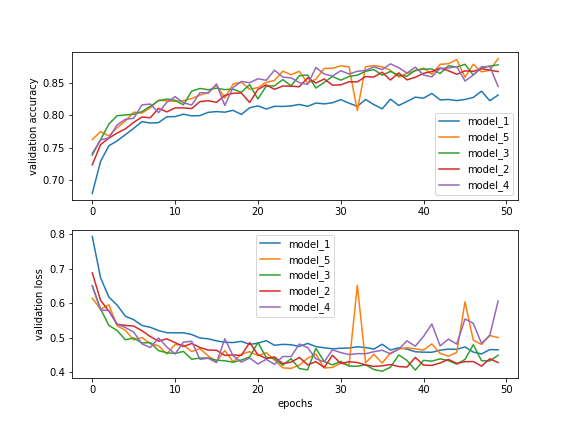
\includegraphics[width=\textwidth]{../notebooks/figures/validation_nn.png}
\caption{Convergencia modelos red neuronal}
\label{fig:nn_convergencia}
\end{figure} 

Vemos que con ese número de \textit{epochs} nuestros modelos convergen sin problema, nuestro Test loss ronda 0.4773907017086763 y test accuracy 0.8876628076115841, veamos ahora ahora el AUC de nuestros modelos en al figura [\ref{fig:nn_auc}], escogemos el segundo modelo ya que parece más estable, y hacemos la validación cruzada con 5 particiones de el mismo donde obtenemos un resultado de \textbf{0.857 (+/- 0.012)}. 

\begin{figure}[H]
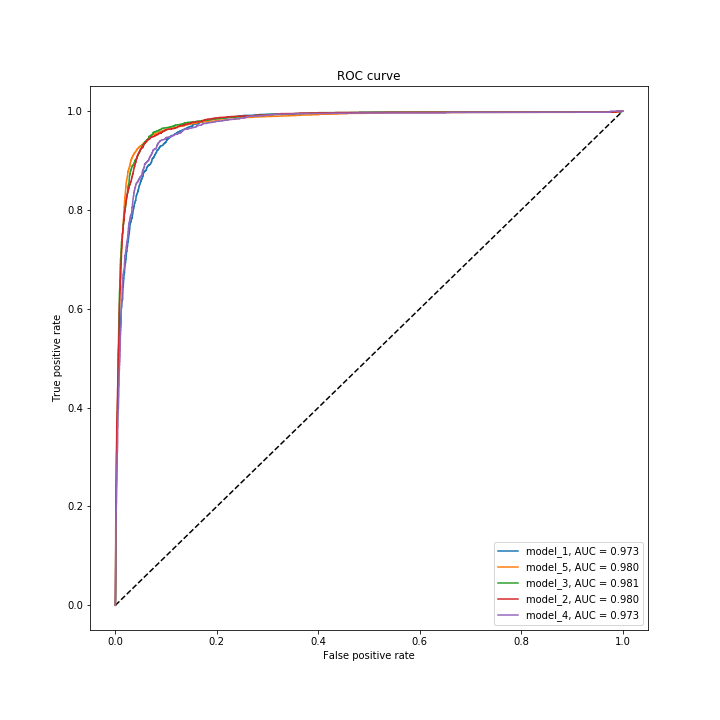
\includegraphics[width=\textwidth]{../notebooks/figures/roc_nn.png}
\caption{AUC ROC red neuronal}
\label{fig:nn_auc}
\end{figure} 

Con esto concluye esta sección respecto a la red neuronal, comprobandola contra nuestro conjunto de test, conseguimos una score de \textbf{0.75}, comparando lo que tarda cada ejecución de la red neuronal, tanto en entrenar, como en encontrar valores óptimos llegamos a la conclusión de que no es rentable para este problema (o tal vez nuestro conjunto de valores elegidos no ha sido el adecuado). Tambien probamos a utilizar BatchNormalization y con otros datos pero no conseguimos mejores resultados y como hemos comentado, el tiempo de ejecución es muy elevado comparado con otros algoritmos (puede llegar a tardar \textbf{horas}), un simple Random Forest Classifier proporciona mejores resultados tardando muchísimo menos.

\section*{Tabla}
\addcontentsline{toc}{section}{Tabla}  

Adjuntamos una foto de nuestras mejores 20 subidas en la figura [\ref{fig:subidas}].

\begin{figure}[H]
\begin{center}
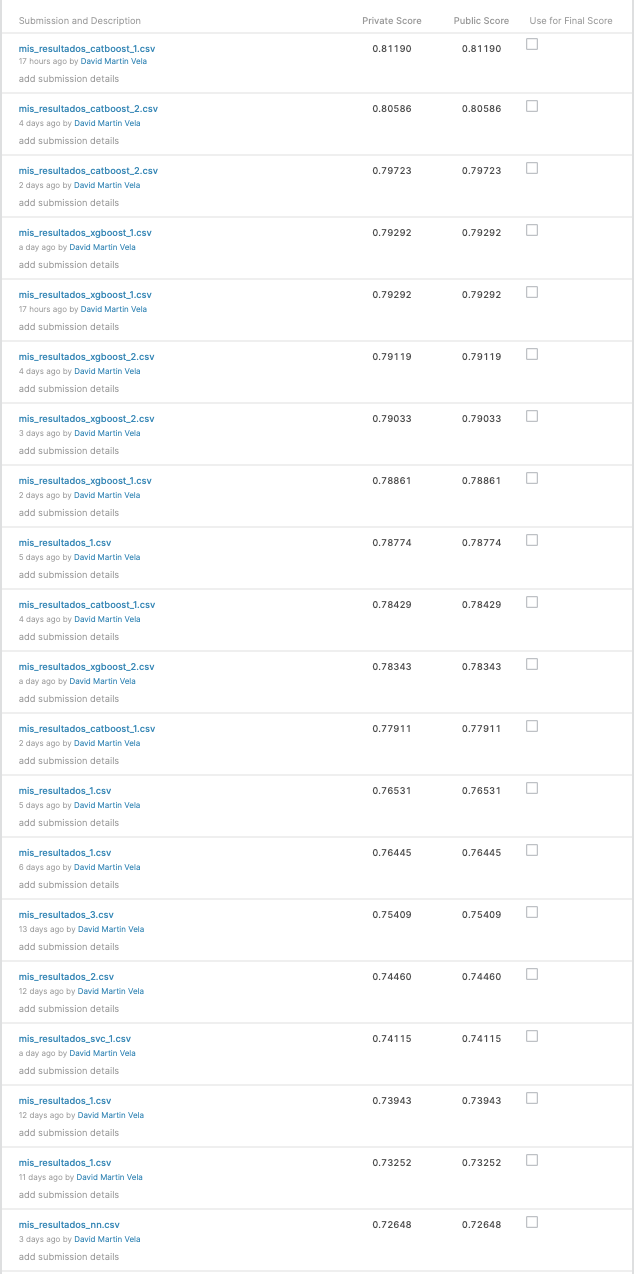
\includegraphics[width=9cm]{../notebooks/figures/subidas.png}
\caption{Subidas a la plataforma Kaggle}
\label{fig:subidas}
\end{center}
\end{figure} 

Todo lo relevante para recrear las subidas se encuentran en el notebook \textbf{vanilla.ipynb}, donde tenemos principalmente dos versiones, una primera versión \textbf{vanilla} (una versión básica donde tratamos los valores perdidos, etiquetamos y pasamos directamente a los modelos) y una segunda versión donde realizamos algo más de preprocesados, la diferencia entre ambas es el tipo de etiquetado (en el primero únicamente usamos label encoding mientras que en el segundo hacemos one hot de otros atributos) y que en la segunda versión podemos tratar con los outliers y skewed data, en ambas versiones tenemos disposibles los preprocesamientos de valores perdidos, podemos ejecutarlos selectivamente en nuestro código dependiendo de la opción que queramos, igual con el tipo de balanceo (SMOTE o RandomOverSampling). La mayoria de métodos relacionados con algoritmo ejecutan un conjunto de todo ellos, y luego se profundizan sobre los que hemos comentado en la sección de algoritmos realizando tuning. De estos que se profundizan se genera un archivo con el nombre de \textbf{mis\_resultados\_\{algoritmo-utilizado\}\_\{versión\}} (Los que no tienen el algoritmo utilizado son los iniciales donde únicamente usaba random forest y la versión). En score train se introduce la puntuación de validación cruzada con métrica accuracy utilizando 5 particiones y en score test la puntuación obtenida en Kaggle. En conclusión, por mucho preprocesamiento que hagamos al final si entendemos y sabemos configurar un algoritmo complejo con los parámetros adecuados podemos alcanzar resultados muy prometedores sin siquiera tener que indagar en el dataset. Al final los preprocesamientos que más diferencias han proporcionado han sido los relacionados con el balance de nuestro conjunto de datos. Cuando nos referimos a \textbf{Tuning} y \textbf{No tuning}, lo que queremos decir es que en un caso se ha realizado un estudio de los parámetros del algoritmo (sea para evitar el sobreajuste por ejemplo ajustado la profundidad) mientras que en el otro se han escogido unos parámetros por defecto que pueden funcionar bien o no. La tabla está ordenada por la puntuación obtenida en el conjunto \textbf{test}, la columna de la posición quiere decir la posición en la que nos encontrabamos en el momento al haber subido el fichero, puede que nuestra subida no fuera muy buena y en cuyo caso seguiríamos teniendo la posición de otra subida en otro momento.

% Please add the following required packages to your document preamble:
% \usepackage{multirow}
% \usepackage{graphicx}
\begin{table}[H]
\centering
\resizebox{\textwidth}{!}{%
\begin{tabular}{|c|c|c|c|c|c|}
\hline
\textbf{Preprocesamiento} & \textbf{Fecha Subida} & \textbf{Posición} & \textbf{Algoritmo} & \textbf{Score Train} & \textbf{Score Test} \\ \hline
\begin{tabular}[c]{@{}c@{}}(V1) Valores perdidos eliminados\\ Etiquetamos con LabelEncoder\\ Balanceo con RandomOverSampling\end{tabular} & 30/12/2020 & 5 & \begin{tabular}[c]{@{}c@{}}Red Neuronal 3 capas densas\\ 1 input layer (relu), 1 hidden layer (relu) y 1 output layer (softmax)\end{tabular} & 0.857 & 0.72648 \\ \hline
\begin{tabular}[c]{@{}c@{}}(V1) Valores perdidos eliminados\\ Etiquetamos con LabelEncoder\\ Balanceo con SMOTE\end{tabular} & 22/12/2020 & 8 & \begin{tabular}[c]{@{}c@{}}(No tuning) RandomForestClassifier()\\ (Sospechamos de overfitting)\\ Accuracy on Training set:  1.0\\ Accuracy on Testing set:  0.9123287671232877\end{tabular} & 0.88739 & 0.73252 \\ \hline
\begin{tabular}[c]{@{}c@{}}(V1) Valores perdidos eliminados\\ Etiquetamos con LabelEncoder\\ Balanceo con SMOTE\end{tabular} & 21/12/2020 & 7 & \begin{tabular}[c]{@{}c@{}}(Tuning) RandomForestClassifier(max\_depth = 9, \\ max\_features = 'auto', min\_samples\_leaf = 1, \\ min\_samples\_split = 15, n\_estimators = 1000)\end{tabular} & 0.84520 & 0.73943 \\ \hline
\begin{tabular}[c]{@{}c@{}}(V1) Valores perdidos eliminados\\ Etiquetamos con LabelEncoder\\ Balanceo con RandomOverSampling\end{tabular} & 01/01/2020 & 5 & \begin{tabular}[c]{@{}c@{}}(Tuning) SVC(kernel = 'rbf', \\ gamma = 'auto', C = 100)\end{tabular} & 0.90312 & 0.74115 \\ \hline
\begin{tabular}[c]{@{}c@{}}(V2) Valores perdidos media y moda\\ Etiquetado de one hot encoding de \\ ciudad, tipo\_marchas, combustible\\ y company. Se elimina Nombre.\\ Balanceo con SMOTE\end{tabular} & 21/12/2020 & 7 & \begin{tabular}[c]{@{}c@{}}(No tuning) RandomForestClassifier()\\ Accuracy on Training set:  1.0\\ Accuracy on Testing set:  0.914349276974416\\ (Sospechamos de overfitting)\end{tabular} & 0.89140 & 0.74460 \\ \hline
\begin{tabular}[c]{@{}c@{}}(V2) Valores perdidos eliminados\\ Etiquetado de one hot encoding de \\ ciudad, tipo\_marchas y combustible,\\ Label encoding Nombre,\\ Skewed data y outliers\\ Balanceo con SMOTE\end{tabular} & 20/12/2020 & 6 & \begin{tabular}[c]{@{}c@{}}(Tuning) RandomForestClassifier(n\_estimators = 1000 \\ min\_samples\_split = 15, \\ min\_samples\_leaf = 1, \\ max\_features = 'auto', \\ max\_depth = 9)\end{tabular} & 0.84455 & 0.75409 \\ \hline
\begin{tabular}[c]{@{}c@{}}(V1) Valores perdidos media y moda\\ Etiquetamos con LabelEncoder\\ Balanceo con SMOTE\end{tabular} & 27/12/2020 & 10 & \begin{tabular}[c]{@{}c@{}}(Tuning) XGBClassifier(subsample = 0.7, n\_estimators = 918, \\ min\_child\_weight = 1,  max\_depth = 7, learning\_rate = 0.15, \\ colsample\_bytree = 1.0)\end{tabular} & 0.90628 & 0.76445 \\ \hline
\begin{tabular}[c]{@{}c@{}}(V1) Valores perdidos eliminados\\ Etiquetamos con LabelEncoder\\ Balanceo con RandomOverSampling\end{tabular} & 28/12/2020 & 7 & \begin{tabular}[c]{@{}c@{}}(No tuning)  RandomForestClassifier()\\ (Sospechamos de overfitting)\\ Accuracy on Training set:  1.0\\ Accuracy on Testing set:  0.9632925472747497\end{tabular} & 0.94841 & 0.76531 \\ \hline
\begin{tabular}[c]{@{}c@{}}(V1) Valores perdidos eliminados\\ Etiquetamos con LabelEncoder\\ Balanceo con SMOTE\end{tabular} & 31/12/2020 & 8 & \begin{tabular}[c]{@{}c@{}}(No tuning) CatBoostClassifier(iterations=1000, \\ learning\_rate=0.1, random\_strength=0.1, \\ depth=7, loss\_function='MultiClass',\\ eval\_metric='Accuracy',\\ leaf\_estimation\_method='Newton')\end{tabular} & 0.94382 & 0.77911 \\ \hline
\begin{tabular}[c]{@{}c@{}}(V2) Valores perdidos eliminados\\ Etiquetamos con one hot Ciudad,\\ Tipo\_marchas, Combustible y Company,\\ Balanceo con RandomOverSampling\end{tabular} & 01/01/2020 & 5 & \begin{tabular}[c]{@{}c@{}}(Tuning) XGBClassifier(subsample = 0.7, \\ n\_estimators = 918,  min\_child\_weight = 1, \\ max\_depth = 8, learning\_rate = 0.15, \\ colsample\_bytree = 1.0)\end{tabular} & 0.93534 & 0.78343 \\ \hline
\begin{tabular}[c]{@{}c@{}}(V1) Valores perdidos eliminados\\ Etiquetamos con LabelEncoder\\ Balanceo con RandomOverSampling\end{tabular} & 29/12/2020 & 7 & \begin{tabular}[c]{@{}c@{}}(No tuning) CatBoostClassifier(iterations=1000, \\ learning\_rate=0.1, random\_strength=0.1, \\ depth=7, loss\_function='MultiClass',\\ eval\_metric='Accuracy',\\ leaf\_estimation\_method='Newton')\end{tabular} & 0.92213 & 0.78429 \\ \hline
\begin{tabular}[c]{@{}c@{}}(V1) Valores perdidos media y moda\\ Etiquetamos con LabelEncoder\\ Balanceo con RandomOverSampling\end{tabular} & 28/12/2020 & 7 & \begin{tabular}[c]{@{}c@{}}(Tuning) XGBClassifier(subsample = 0.7, \\ n\_estimators = 918,  min\_child\_weight = 1, \\ max\_depth = 8, learning\_rate = 0.15, \\ colsample\_bytree = 1.0)\end{tabular} & 0.85165 & 0.78774 \\ \hline
\begin{tabular}[c]{@{}c@{}}(V1) Valores perdidos eliminados\\ Etiquetamos con LabelEncoder\\ Balanceo con RandomOverSampling\end{tabular} & 31/12/2020 & 7 & \begin{tabular}[c]{@{}c@{}}(Tuning) XGBClassifier(subsample = 0.7, \\ n\_estimators = 918,  min\_child\_weight = 1, \\ max\_depth = 8, learning\_rate = 0.15, \\ colsample\_bytree = 1.0)\end{tabular} & 0.94716 & 0.78861 \\ \hline
\begin{tabular}[c]{@{}c@{}}(V2) Valores perdidos moda Company\\ Etiquetamos con one hot Ciudad,\\ Tipo\_marchas y Combustible,\\ Label encoding Nombre,\\ Skewed data y outliers,\\ Balanceo con RandomOverSampling\end{tabular} & 30/12/2020 & 7 & \begin{tabular}[c]{@{}c@{}}(Tuning) XGBClassifier(subsample = 0.7, \\ n\_estimators = 918, min\_child\_weight = 1,  \\ max\_depth = 7, learning\_rate = 0.15, \\ colsample\_bytree = 1.0)\\ (Posible overfitting)\\ Accuracy on Training set:  1.0\\ Accuracy on Testing set:  0.9624481438489293\end{tabular} & 0.94952 & 0.79033 \\ \hline
\begin{tabular}[c]{@{}c@{}}(V2) Valores perdidos eliminados\\ Etiquetamos con one hot Ciudad,\\ Tipo\_marchas y Combustible\\ Label encoding Nombre,\\ Skewed data y outliers,\\ Balanceo con RandomOverSampling\end{tabular} & 29/12/2020 & 7 & \begin{tabular}[c]{@{}c@{}}(Tuning) XGBClassifier(subsample = 0.7, \\ n\_estimators = 918, min\_child\_weight = 1,  \\ max\_depth = 9, learning\_rate = 0.15, \\ colsample\_bytree = 1.0)\end{tabular} & 0.95244 & 0.79119 \\ \hline
\begin{tabular}[c]{@{}c@{}}(V1) Valores perdidos moda Company,\\ Etiquetamos con LabelEncoder,\\ Balanceo con RandomOverSampling\end{tabular} & 01/01/2021 & 5 & \begin{tabular}[c]{@{}c@{}}(Tuning) XGBClassifier(subsample = 0.7, n\_estimators = 918, \\ min\_child\_weight = 1,  max\_depth = 8, learning\_rate = 0.15, \\ colsample\_bytree = 1.0)\end{tabular} & 0.94595 & 0.79292 \\ \hline
\begin{tabular}[c]{@{}c@{}}(V2) Valores perdidos moda Company, \\ Etiquetamos con one hot Ciudad,\\ Tipo\_marchas y Combustible\\ Skewed data y outliers,\\ Balanceo con RandomOverSampling\end{tabular} & 31/12/2020 & 5 & \begin{tabular}[c]{@{}c@{}}(No tuning) CatBoostClassifier(iterations=1000, learning\_rate=0.1,\\ random\_strength=0.1, depth=7, loss\_function='MultiClass',\\ eval\_metric='Accuracy',leaf\_estimation\_method='Newton')\end{tabular} & 0.94586 & 0.79723 \\ \hline
\begin{tabular}[c]{@{}c@{}}(V2) Valores perdidos eliminados\\ Etiquetamos con one hot Ciudad,\\ Tipo\_marchas y Combustible\\ Label encoding Nombre,\\ Skewed data y outliers,\\ Balanceo con RandomOverSampling\end{tabular} & 29/12/2020 & 5 & \begin{tabular}[c]{@{}c@{}}(Tuning) CatBoostClassifier(depth = 10, one\_hot\_max\_size = 2, \\ iterations = 800, random\_strength = 0.03, learning\_rate = 0.1,\\     od\_type = 'IncToDec', loss\_function='MultiClass', eval\_metric='Accuracy',\\     leaf\_estimation\_method='Newton')\end{tabular} & 0.94650 & 0.80586 \\ \hline
\multirow{3}{*}{\begin{tabular}[c]{@{}c@{}}(V1) Valores perdidos media y moda\\ Etiquetamos con LabelEncoder\\ Balanceo con RandomOverSampling\end{tabular}} & \multirow{3}{*}{-} & \multirow{3}{*}{-} & \multirow{3}{*}{\begin{tabular}[c]{@{}c@{}}(Tuning) CatBoostClassifier(depth = 10, one\_hot\_max\_size = 2, \\ iterations = 800, random\_strength = 0.03, learning\_rate = 0.1, od\_type = 'IncToDec', \\ loss\_function='MultiClass', eval\_metric='Accuracy', leaf\_estimation\_method='Newton')\end{tabular}} & \multirow{3}{*}{0.93758} & \multirow{3}{*}{0.81190} \\
 &  &  &  &  &  \\
 &  &  &  &  &  \\ \hline
\end{tabular}%
}
\caption{Tabla de puntuaciones}
\label{tab:tabla-scores}
\end{table}

%\caption{Tabla de puntuaciones}
%\label{tab:tabla-scores}


%% bibliography
\medskip

\printbibliography[
heading=bibintoc,
title={Referencias}
]


\end{document}
